% !TeX root = Applied Graph Theory.tex

\title{\textbf{Applied Graph Theory}}

\date{}
\maketitle

\begingroup
\let\clearpage\relax
\tableofcontents
\endgroup

\clearpage

\renewcommand{\nomname}{List of Symbols}
\nomenclature[01]{$V(G)$}{Vertex set of graph $G$}
\nomenclature[02]{$E(G)$}{Edge set of graph $G$}
\nomenclature[03]{$\sim$}{is adjacenct to}
\nomenclature[04]{$\deg(v)$}{Degree of vertex $v$}
\nomenclature[05]{$\ecc(v)$}{Eccentricity of vertex $v$}
\nomenclature[06]{$\rad(G)$}{Radius of graph $G$}
\nomenclature[07]{$\diam(G)$}{Diameter of graph $G$}
\nomenclature[08]{$A(G)$}{Adjacency matrix graph $G$}

\nomenclature[10]{$G - v$}{Graph obtained from $G$ by deleting vertex $v$ and all edges incident with $v$}
\nomenclature[11]{$G - e$}{Graph obtained from $G$ by deleting edge $e$}

\nomenclature[20]{$K_n$}{Complete graph of order $n$ (size $\binom{n}{2}$)}
\nomenclature[21]{$P_n$}{Path graph of order $n$ (size $n - 1$)}
\nomenclature[22]{$C_n$}{Cycle graph of order $n$ (size $n$)}

\nomenclature[30]{$L(G)$}{Line graph of $G$}
\printnomenclature[10em]

\clearpage

\section{Introduction}\label{sec:Intro}
A \newterm{graph} is an ordered pair $G = (V, E)$ where $V$ is a nonempty set called the \newterm{vertex set}, whose elements are the \newterm{vertices} of $G$, and $E$ is a set of unordered pairs of distinct vertices of $G$, whose elements are the \newterm{edges} of $G$. The \newterm{order} of $G$ is its number of vertices and the \newterm{size} of $G$ is its number of edges.

Two vertices $u$ and $v$ of $G$ are \newterm{adjacent}, denoted by $u \sim v$, if $(u,v) \in E$ -- we may also denote the edge $(u,v)$ as simply $uv$. Note that $uv = vu$. If there is no edge between $u$ and $v$, then they are \newterm{nonadjacent}, denoted by $u \nsim v$. The vertex $v$ and the edge $uv$ are said to be \newterm{incident} with each other. The \newterm{degree} of a vertex $v$ is the number of edges incident with it, or equivalently, the number of vertices adjacent with it, and is denoted by $\deg(v)$.

\begin{Lemma}[Handshaking Lemma]
The sum of the degrees of all vertices of a graph is twice its size.
\end{Lemma}

\begin{proof}
Let $G$ be a graph, and consider the sum of its degrees, $\sum_{v \in V(G)} \deg v$. As each edge is incident with exactly two vertices, each edge is counted once by two terms in this summation. Thus, the sum is equal to twice the number of edges.
\end{proof}

\begin{Corollary}
The number of vertices of odd degree in a graph is always even.
\end{Corollary}

\begin{proof}
Let $G$ be a graph. We know that
\begin{equation}
\sum_{v \in V(G)} \deg v = 2 |E(G)|. \label{eq:deg-sum}
\end{equation}
Considering the vertices of odd and even degrees, we can write \eqref{eq:deg-sum} as
\begin{equation}
\sum_{v \in V(G) : \deg v\ \text{odd}} \deg v + \sum_{v \in V(G) : \deg v\ \text{even}} \deg v = 2 |E(G)|.
\end{equation}
Both the second term on the LHS and the RHS are even integers, and therefore so is the first term on the LHS. But a sum of odd integers is even only if the number of terms is even. Thus, $G$ has an even number of vertices of odd degree.
\end{proof}

A \newterm{regular graph} is a graph in which all vertices have the same degree. This common value of the degree is the \newterm{regularity} of the graph. A regular graph of regularity $k$ is a \newterm{$k$-regular} graph. A \newterm{cubic} graph is a $3$-regular graph.

\begin{Exercise}
Prove that any cubic graph has even order. For what other order(s) will this statement hold?
\end{Exercise}

\begin{Theorem}
In any graph on two or more vertices, at least two vertices have the same degree.
\end{Theorem}

\begin{proof}
Let $G$ be a graph of order $n \ge 2$. The minimum possible degree of a vertex of $G$ is $0$, and the maximum possible degree is $n - 1$ (as there are only $n$ vertices in $G$). Thus, in order for the $n$ vertices of $G$ to have different degrees, the $n$ different degrees must be exactly $0, 1, \ldots, n - 1$. But if some vertex of $G$ has degree $n - 1$, then it is adjacent to all other vertices, and therefore $G$ cannot have a vertex of degree $0$. Thus, at least two vertices of $G$ have the same degree.
\end{proof}

\section{Cartesian Products}\label{sec:CartProds}

The \newterm{Cartesian product} of two graphs $G$ and $H$ is the graph denoted by $G \times H$, whose vertex set is $V(G) \times V(H)$ (the Cartesian product of the vertex sets $V(G)$ and $V(H)$, consisting of all ordered pairs $(u, v)$ where $u$ is a vertex of $G$ and $v$ is a vertex of $H$), in which two vertices $(u_1, v_1)$ and $(u_2, v_2)$ are adjacent if and only if either $u_1 = u_2$ and $v_1 \sim v_2$ or $u_1 \sim u_2$ and $v_1 = v_2$.

\begin{Exercise}
Prove that if $G$ is a graph of order $p_1$ and size $q_1$, and $H$ is a graph of order $p_2$ and size $q_2$, then $G \times H$ is a graph of order $p_1 p_2$ and size $p_1 q_2 + p_2 q_1$.
\end{Exercise}

\begin{Solution*}
By definition, the vertex set of $G \times H$ is the Cartesian product $V(G) \times V(H)$ of the vertex sets of $G$ and $H$, and therefore contains $|V(G)| \times |V(H)|$ elements. Thus, the order of $G \times H$ is $p_1 p_2$.

Now, consider any vertex $(u, v)$ of $G \times H$. Corresponding to every vertex $u'$ adjacent to $u$ in $G$, there is an edge from $(u, v)$ to $(u', v))$ in $G \times H$. Similarly, corresponding to every vertex $v'$ adjacent to $v$ in $H$, there is an edge from $(u, v)$ from $(u, v')$ in $G \times H$. Thus, the degree of $(u, v)$ in $G \times H$ is $\deg u + \deg v$. Hence, by the Handshaking Lemma, the size of $G \times H$ is half the sum of its vertex degrees, which is
\begin{align*}
\frac 1 2 \sum_{u \in V(G), v \in V(H)} (\deg u + \deg v) & = \frac 1 2 \sum_{u \in V(G), v \in V(H)} \deg u + \frac 1 2 \sum_{u \in V(G), v \in V(H)} \deg v \\
& = p_2 \pqty{\frac 1 2 \sum_{u \in V(G)} \deg u} + p_1 \pqty{\frac 1 2 \sum_{v \in V(H)} \deg v} \\
& = p_2 q_1 + p_1 q_2.
\end{align*}
\end{Solution*}

\begin{Exercise}
Show that if $G$ is an $r$-regular graph and $H$ is an $s$-regular graph, then $G \times H$ is a regular graph of regularity $r + s$.
\end{Exercise}

\section{Subgraphs and Complements}\label{sec:Subgraphs}

A \newterm{subgraph} of a graph $G$ is a graph $H$ whose vertex and edge sets are, respectively, subsets of the vertex and edge sets of $G$ -- i.e., $V(H) \subseteq V(G)$ and $E(H) \subseteq E(G)$. A \newterm{spanning subgraph} of $G$ is a subgraph containing all the vertices of $G$. A subgraph $H$ of a graph $G$ is an \newterm{induced subgraph} if for all vertices $u, v \in V(H)$, $uv \in E(H)$ whenever $uv \in E(G)$ -- i.e., every edge of $G$ that joins two vertices of $H$ is present in $H$.

\begin{Example}\label{ex:Subgraphs}
\cref{fig:Subgraphs} shows a graph $G$ and three subgraphs $H_1$, $H_2$, and $H_3$ of $G$. The subgraph $H_1$ is neither a spanning subgraph (e.g. it does not contain $v_3$), nor an induced subgraph (e.g. it contains vertices $v_2$ and $v_5$ of $G$ but not the edge $v_2 v_5$). $H_2$ is a spanning subgraph and $H_3$ is an induced subgraph of $G$.
\begin{figure}[!htbp]
\centering
\subcaptionbox{$G$\label{fig:SubgraphsG}}{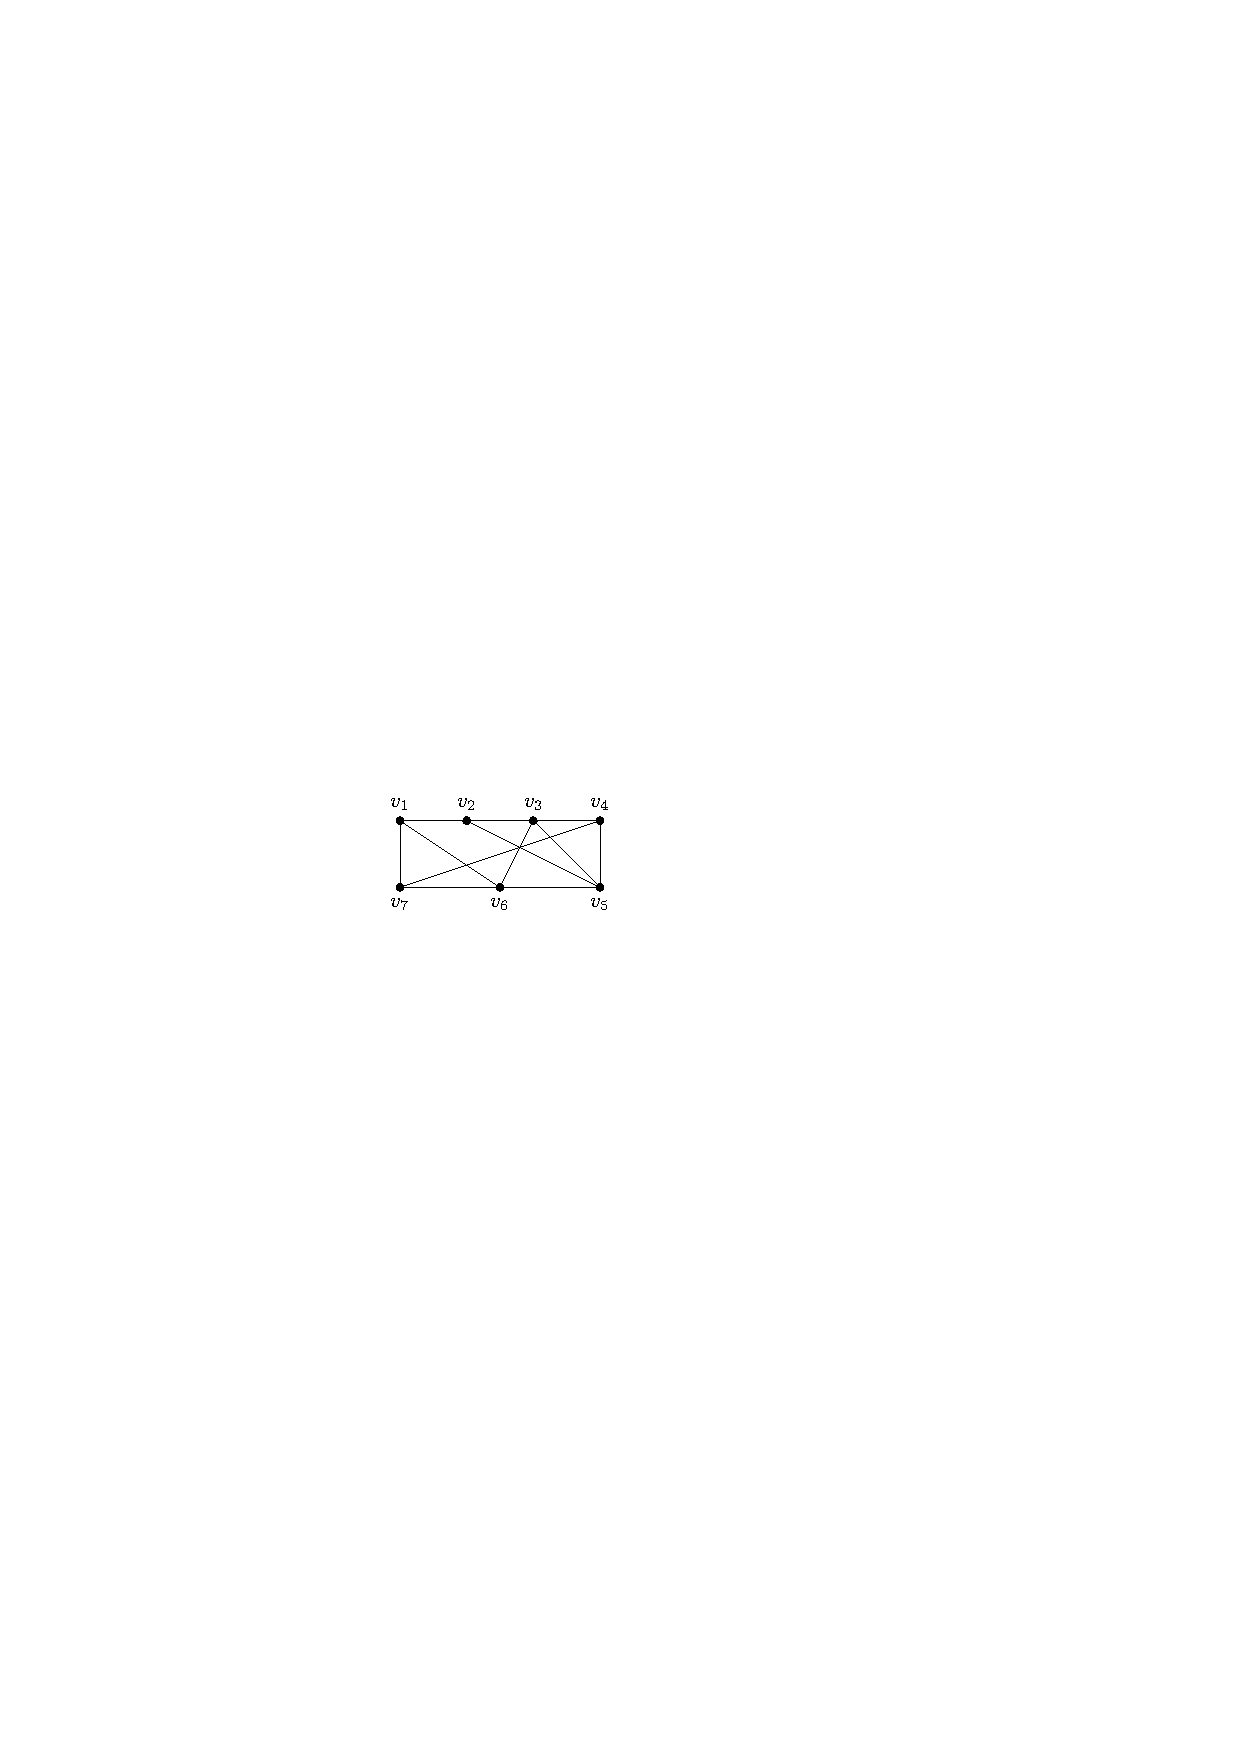
\includegraphics{Images/Subgraphs-G.pdf}} \hfill
\subcaptionbox{$H_1$\label{fig:SubgraphsH1}}{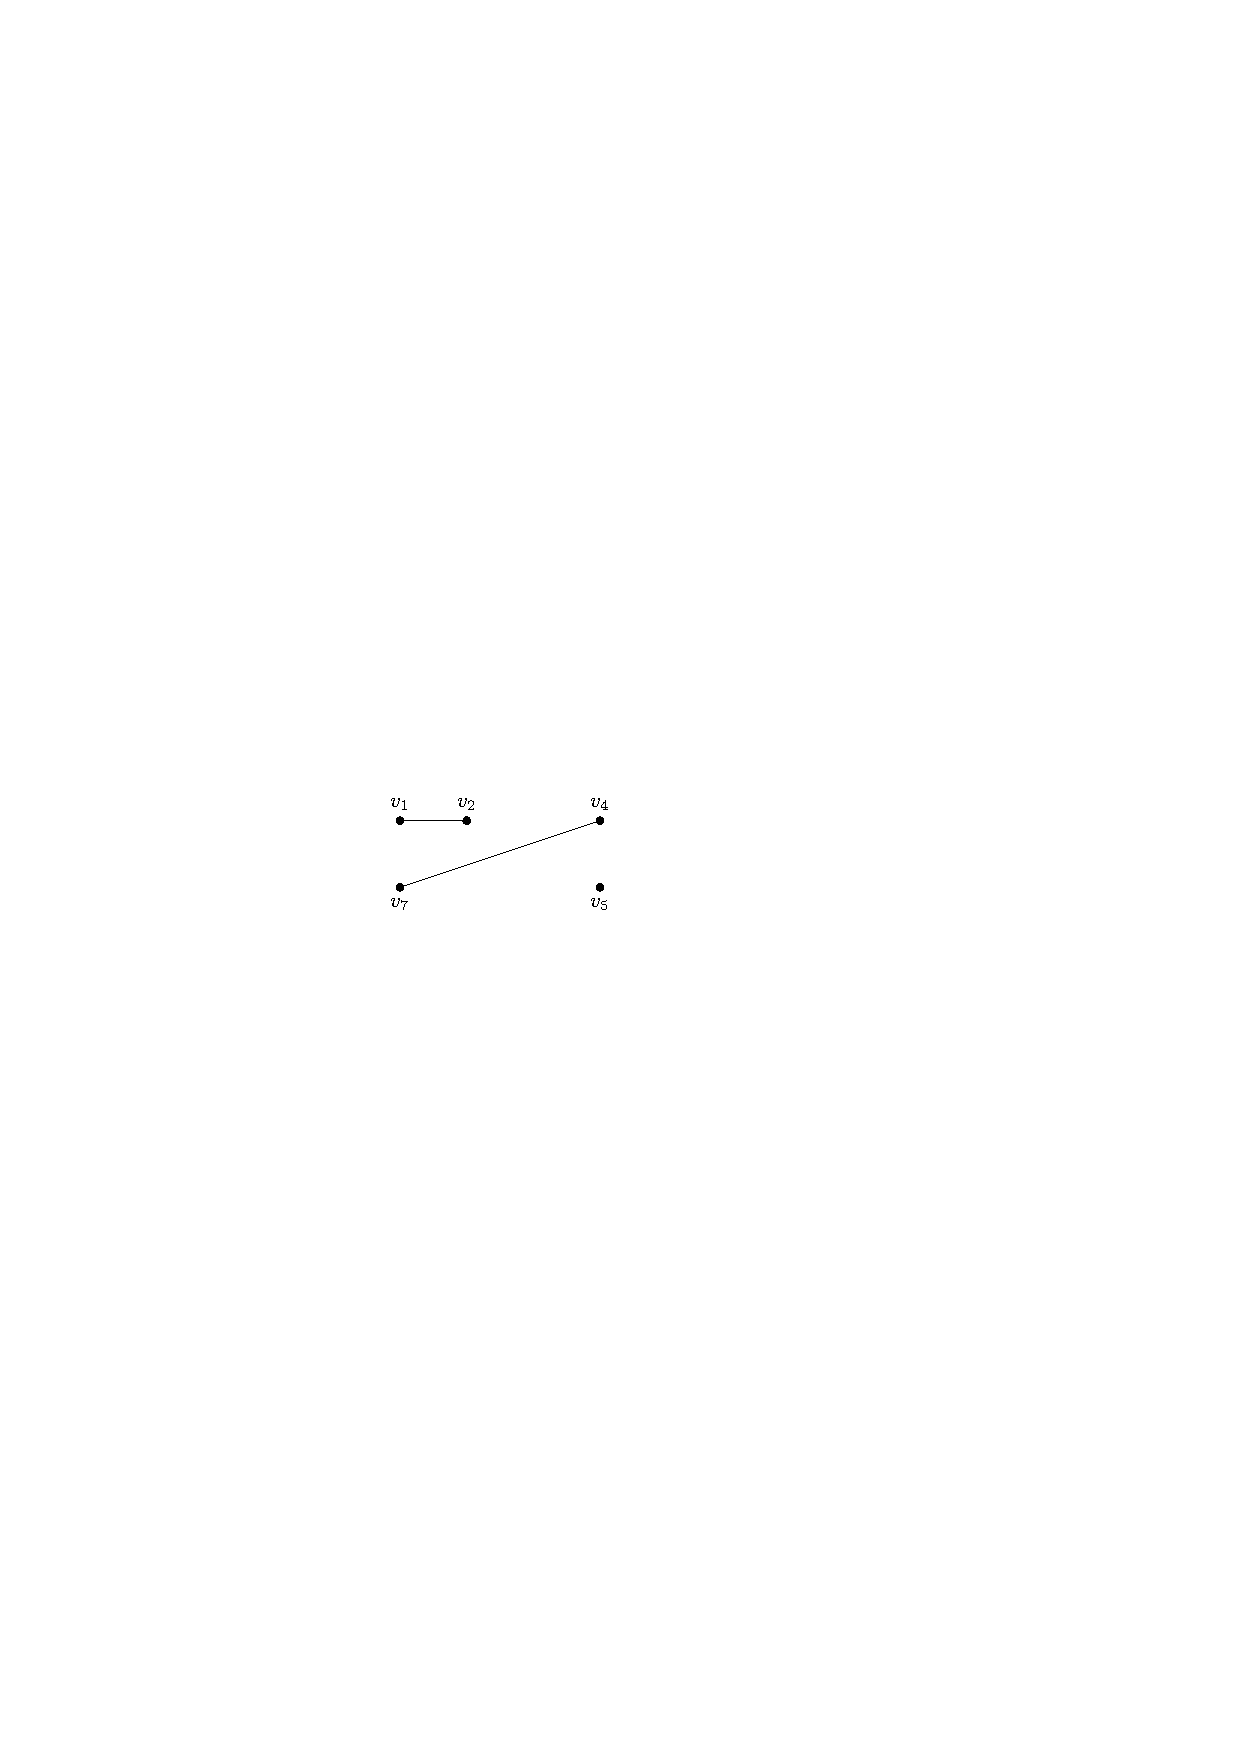
\includegraphics{Images/Subgraphs-H1.pdf}} \hfill
\subcaptionbox{$H_2$\label{fig:SubgraphsH2}}{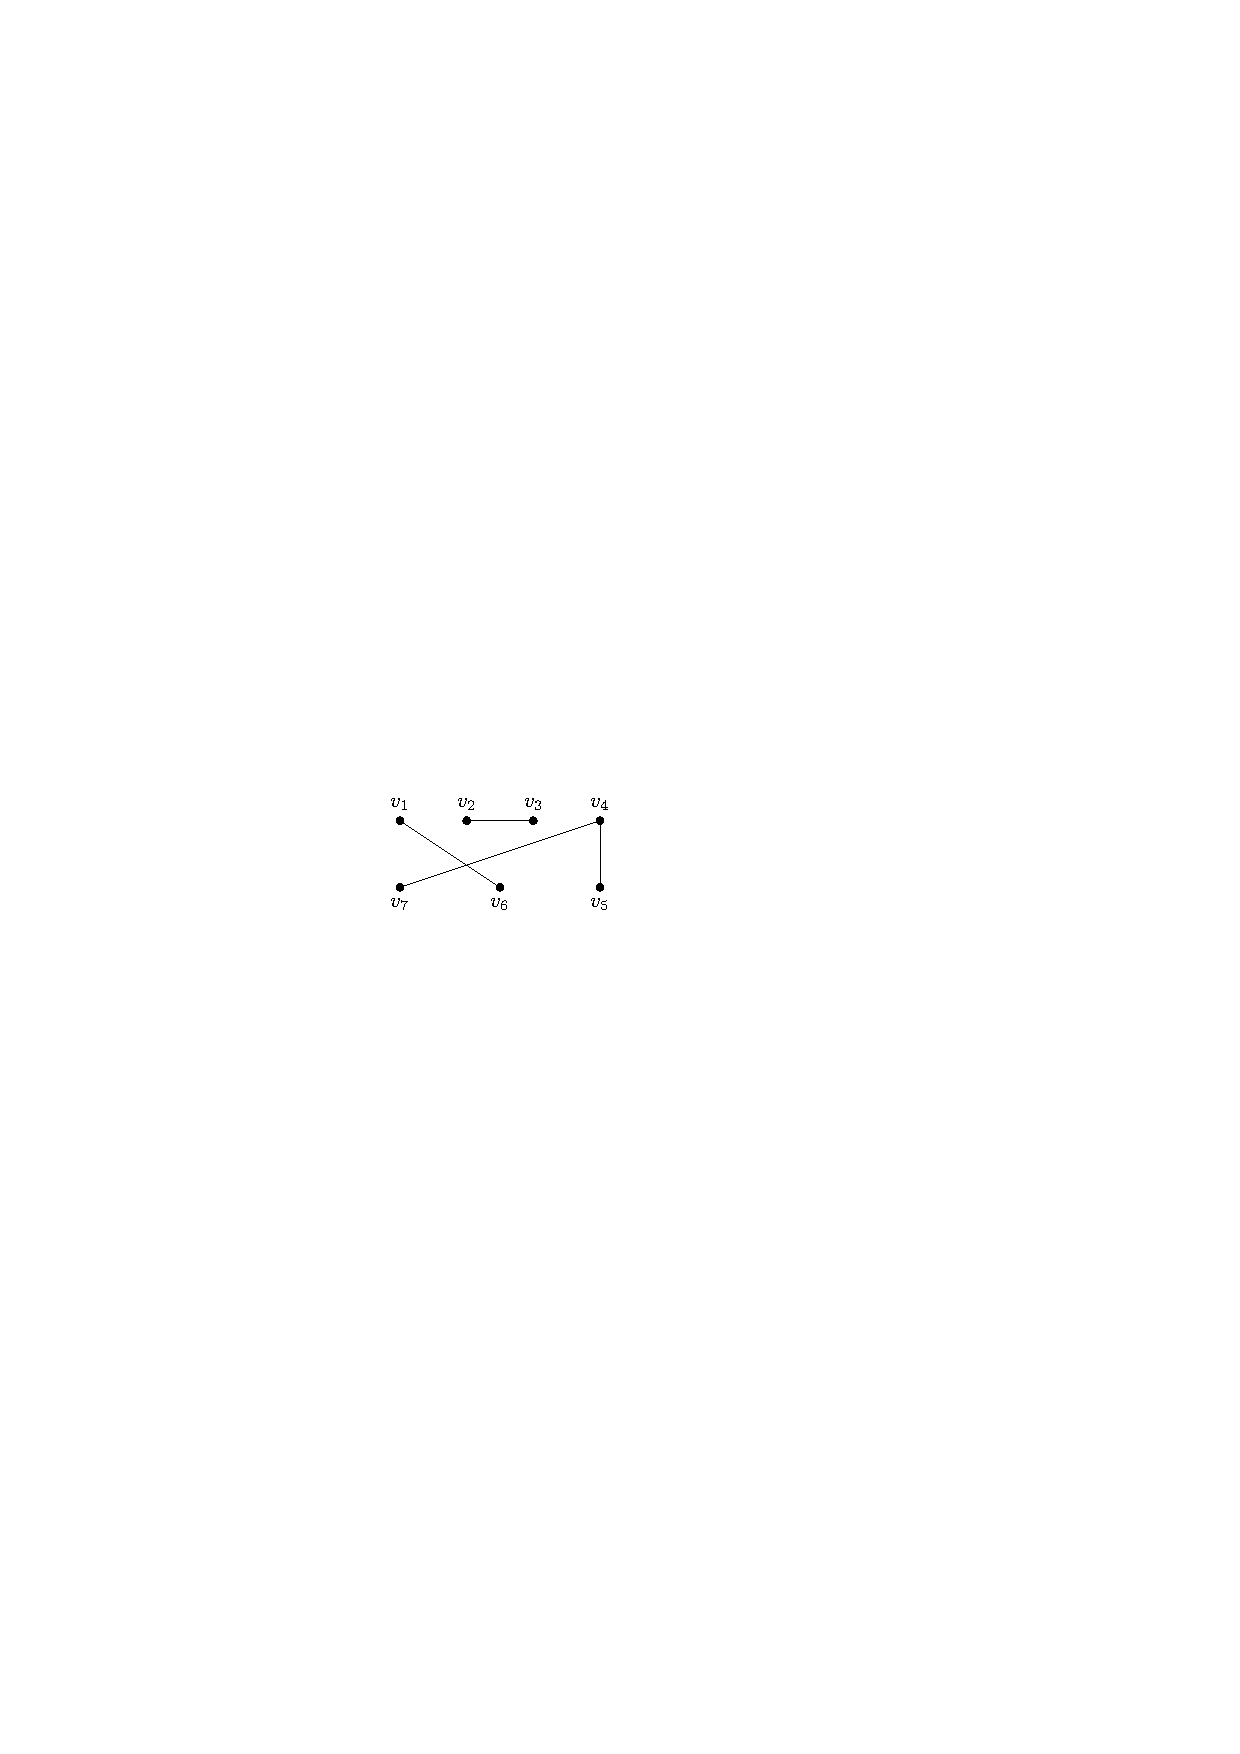
\includegraphics{Images/Subgraphs-H2.pdf}} \hfill
\subcaptionbox{$H_3$\label{fig:SubgraphsH3}}{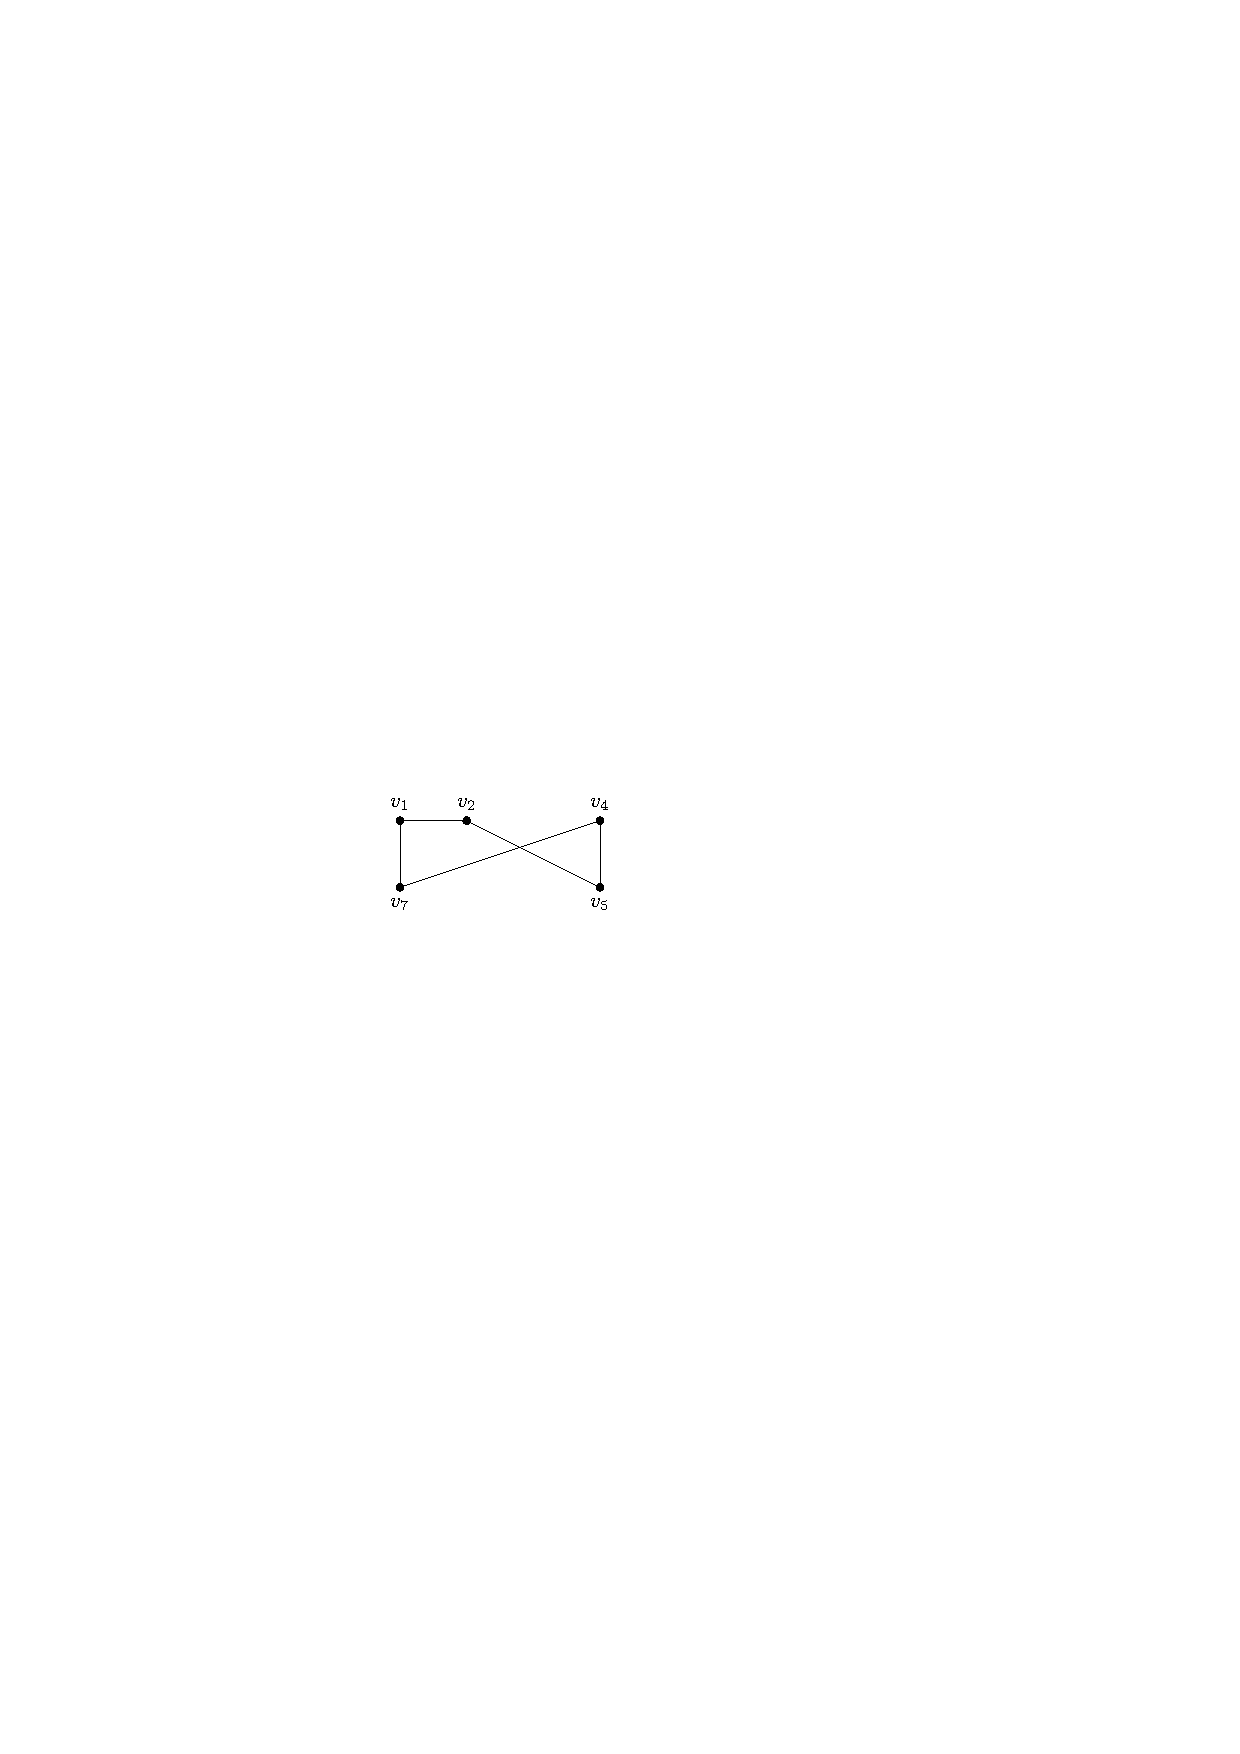
\includegraphics{Images/Subgraphs-H3.pdf}}
\caption{A graph with three of its subgraphs}\label{fig:Subgraphs}
\end{figure}
\end{Example}

A graph is \newterm{complete} if all its vertices are adjacent to one another. The complete graph of order $n$ is denoted by $K_n$. As there is an edge between every pair of distinct vertices of $K_n$, the size of $K_n$ is $\binom n 2$. The \newterm{totally disconnected graph} of order $n$, denoted by $\overline{K_n}$ is the graph of order $n$ that has no edges.

The \newterm{complement} of a graph $G$ is the graph $\overline G$ with the same vertices as $G$, in which any two vertices $u$ and $v$ are adjacent if and only if they are non-adjacent in $G$. Thus, if $G$ is an $(n, m)$-graph, then $\overline G$ is an $\pqty{n, \binom n 2 - m}$-graph. Observe that $\overline K_n$ is (as the notation suggests) the complement of $K_n$.

\begin{Exercise}
If $G$ is a graph of order $n$, and $\deg_G v = k$, what is $\deg_{\overline G} v$?
\end{Exercise}

\begin{Exercise}
Show that if $G$ and $\overline G$ are regular graphs of order $n$ with the same regularity, then the regularity is even and $n = 4t + 1$ for some integer $t$.
\end{Exercise}

\section{Walks, Paths, and Cycles}\label{sec:Walks}

A \newterm{walk} in a simple graph $G$ is a sequence of vertices $v_1, v_2, \ldots, v_k$ such that $v_i \sim v_{i + 1}$ for $i = 1, 2, \ldots, k - 1$. This is a walk \newterm{from $v_1$ to $v_k$} or \newterm{between $v_1$ and $v_k$}, having \newterm{length} $k - 1$. We may also say that this is a walk of length $k - 1$ starting at $v_1$ and ending at $v_k$.

A walk in which no vertex is repeated is a \newterm{path}. Note that the length of a path is the number of edges in it.

A \newterm{closed walk} in $G$ is a walk starting and ending at the same vertex. A closed walk in which no vertex is repeated is a \newterm{cycle}. The length of a cycle is also equal to the number of vertices in it. A cycle of the form $v_1, \ldots, v_{k-1}, v_k$ is usually referred to as ``the cycle $v_1, \ldots, v_{k-1}$''.

\begin{Example}\label{ex:Walk}
Consider the graph $G$ shown below.

\begin{center}
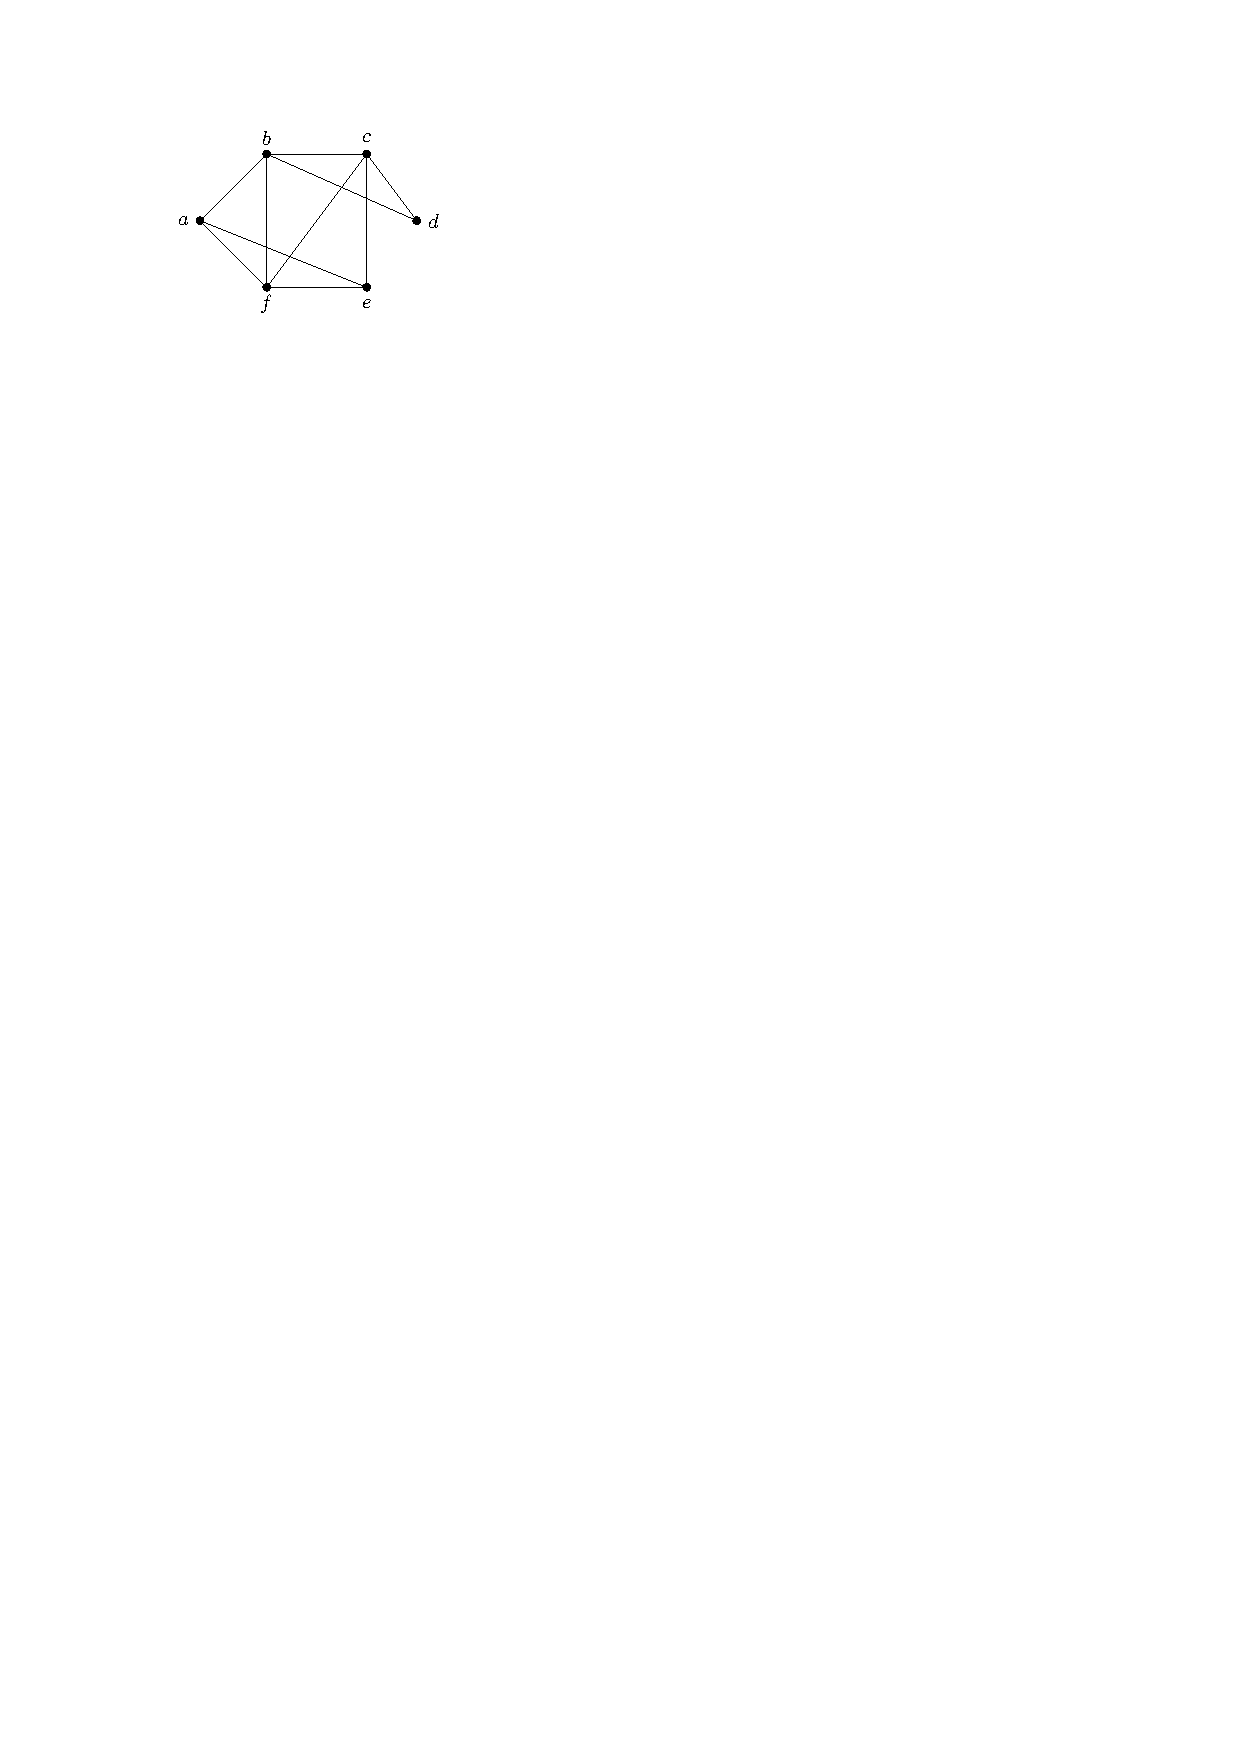
\includegraphics{Images/Walks.pdf}
\end{center}
A walk of length $5$ from $b$ to $c$ in $G$ is $b, f, e, a, e, c$.

\begin{center}
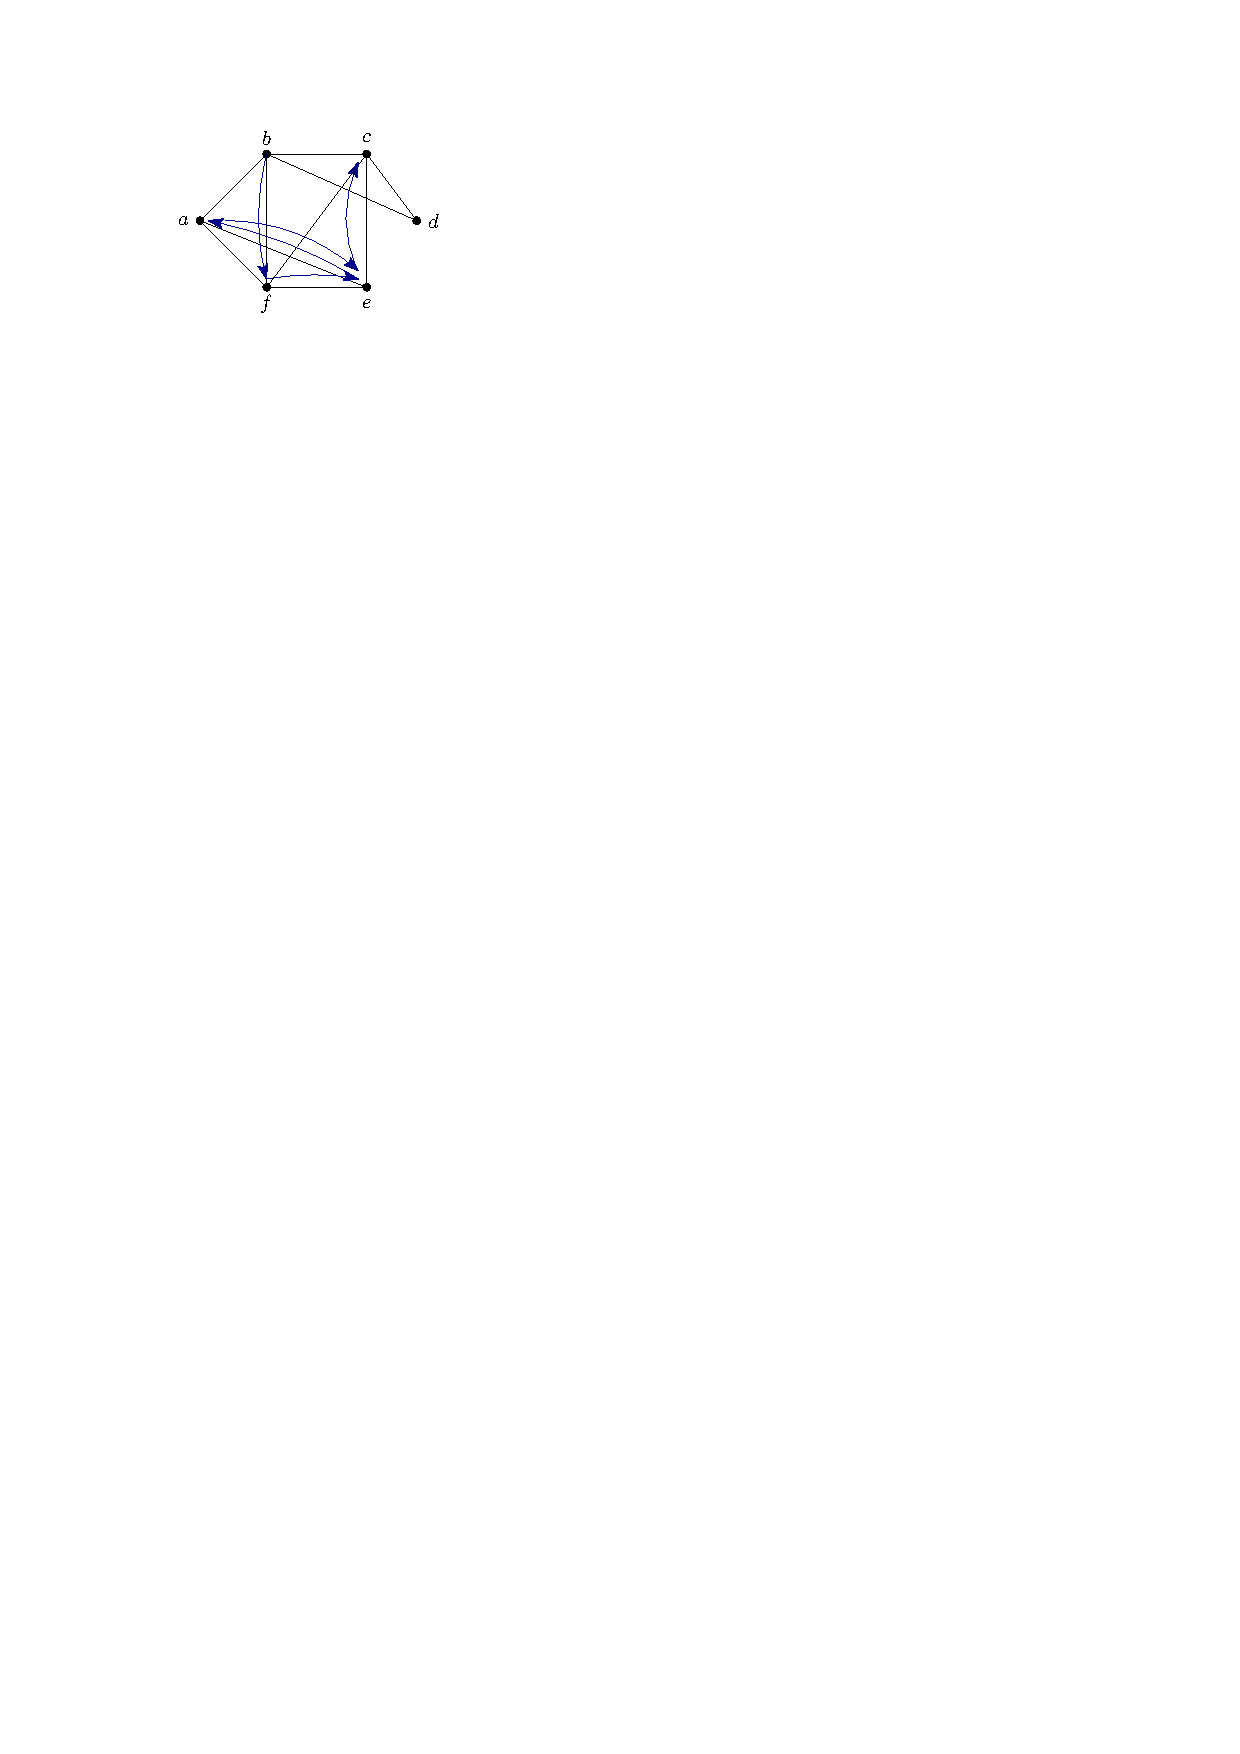
\includegraphics{Images/Walk1.pdf}
\end{center}
This walk is not a path, since the vertex $e$ is repeated. An example of a path from $b$ to $c$ in the same graph $G$ is $b, f, e, c$. The length of this path is $3$.

\begin{center}
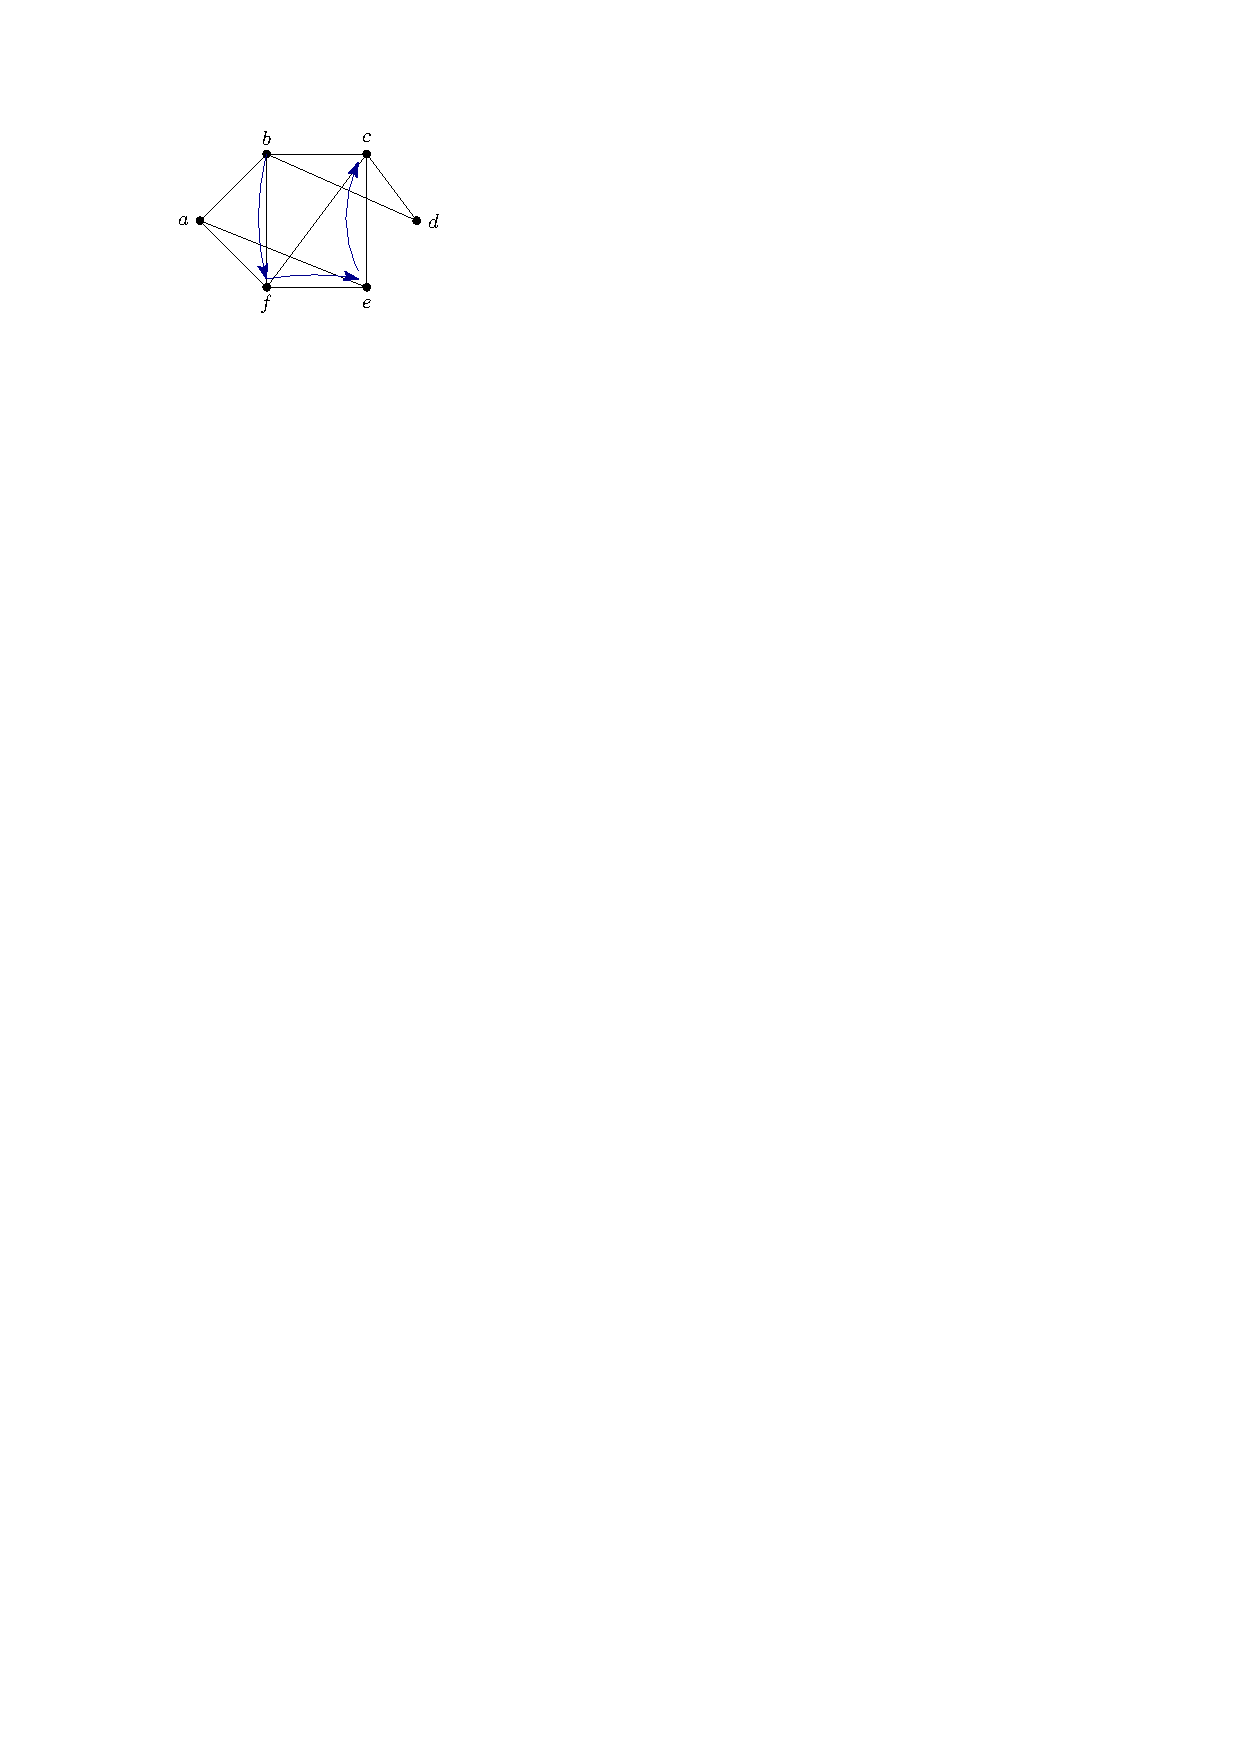
\includegraphics{Images/Path1.pdf}
\end{center}
A cycle of length $4$ in $G$ is $b, f, e, c, b$.

\begin{center}
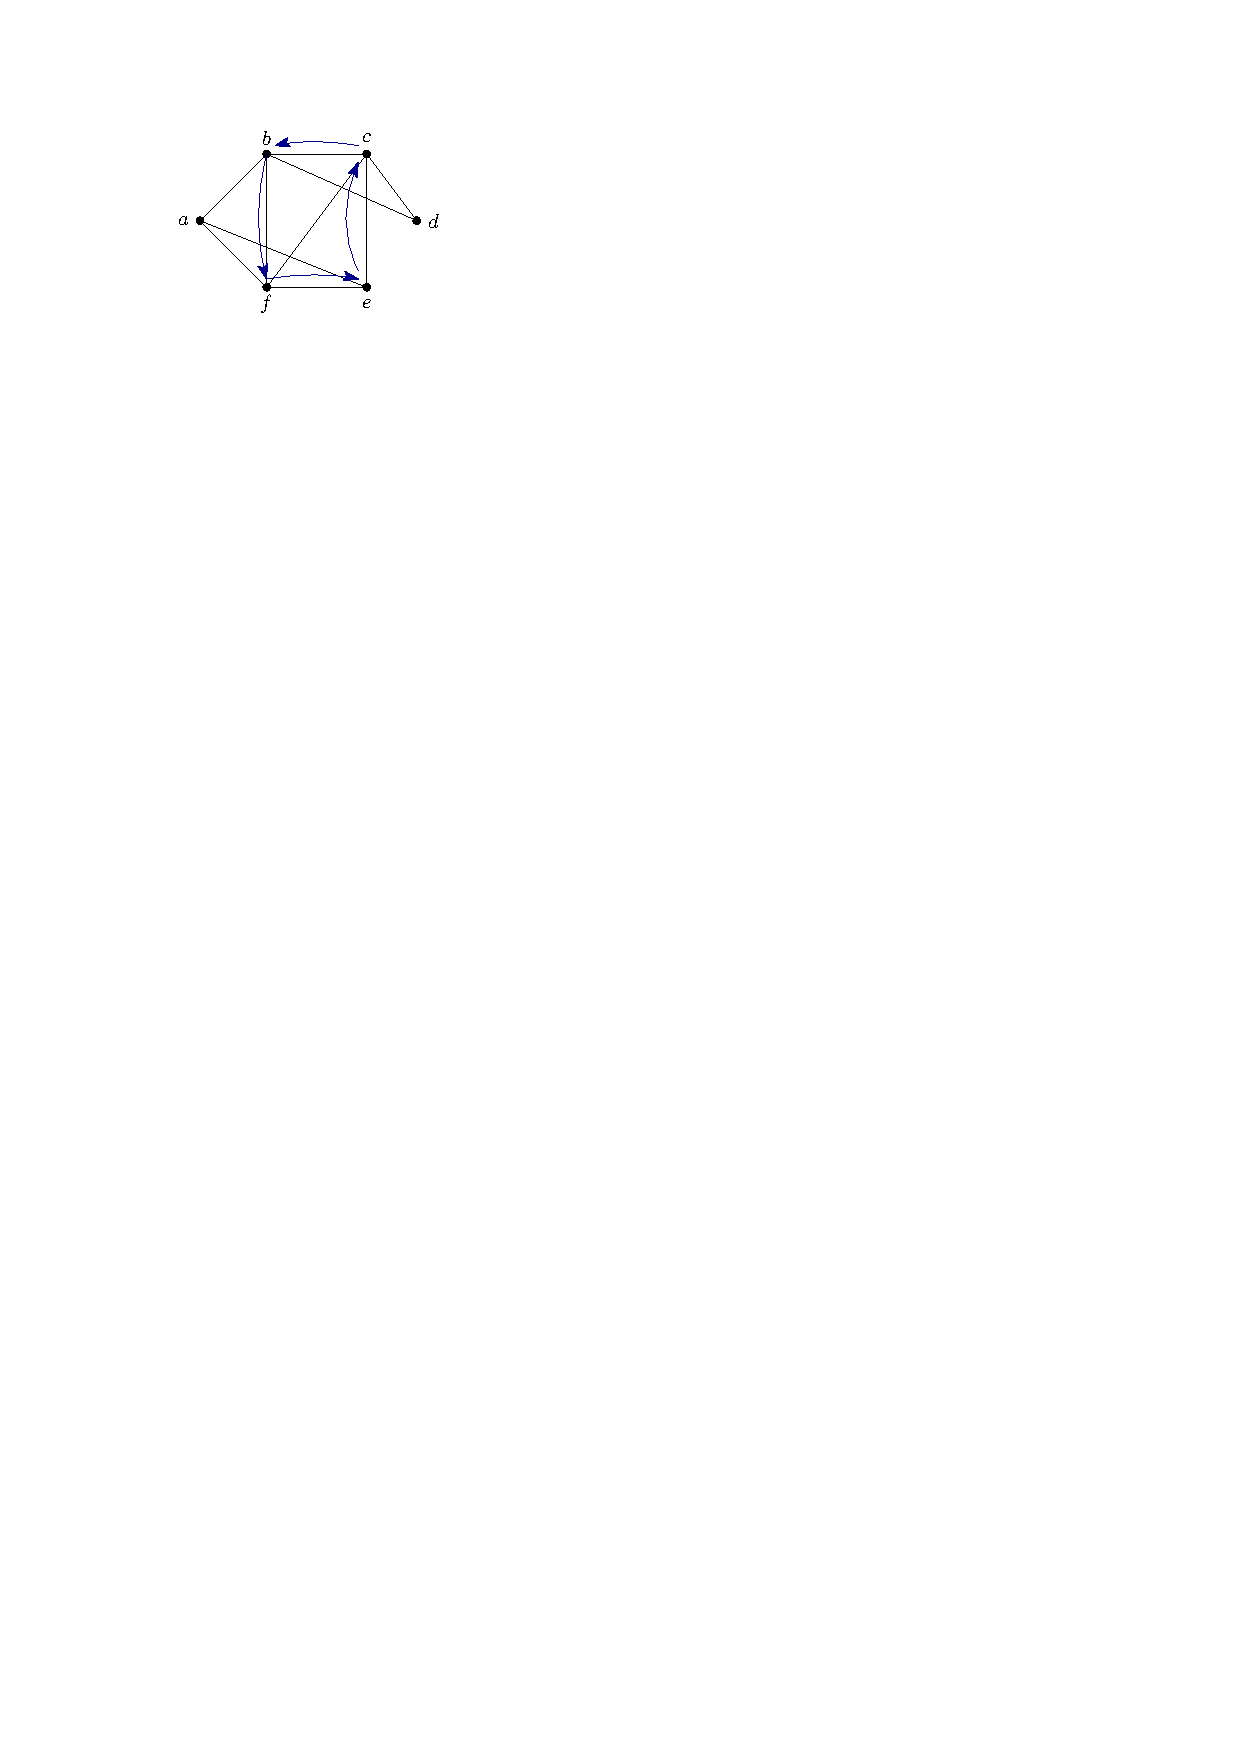
\includegraphics{Images/Cycle1.pdf}
\end{center}
\end{Example}

\section{Distances}\label{sec:Distances}

The \newterm{distance} between two vertices $u$ and $v$ of a graph $G$ is the length of a shortest path between $u$ and $v$ -- such a shortest path between $u$ and $v$ is a \newterm{geodesic} from $u$ to $v$. Thus, the distance between $u$ and $v$ in $G$, denoted by $d_G(u, v)$ is the length of a geodesic from $u$ to $v$ in $G$. When the graph $G$ is clear from the context, we will write $d_G(u, v)$ as $d(u, v)$.

The \newterm{eccentricity} of a vertex $v$, denoted by $\ecc(v)$, is the maximum of all distances from $v$ to any other vertex. That is,
\begin{equation*}
    \ecc(v) = \max_{u \in V(G)} d(u, v) .
\end{equation*}

The \newterm{diameter} of $G$ is the maximum of the eccentricities of vertices of $G$, and the \newterm{radius} of $G$ is the minimum of the eccentricities of vertices of $G$. They are denoted by $\diam(G)$ and $\rad(G)$ respectively. Thus,
\begin{align*}
    \diam(G) & = \max_{v \in V(G)} \ecc(v)= \max_{u, v \in V(G)} d(u, v) \\
    \rad(G) & = \min_{v \in V(G)}\ecc(v) = \min_{v \in V(G)} \max_{u \in V(G)} d(u, v).
\end{align*}

The set of all vertices of $G$ having minimum eccentricity, i.e., the set of all $v \in V(G)$ such that $\ecc v = \rad G$, is the \newterm{centre} of $G$.

\section{Connectedness}\label{sec:Connectedness}

A graph is \newterm{connected} if there is a path between every two of its vertices. Otherwise, it is \newterm{disconnected}. A \newterm{(connected) component} of a graph $G$ is a maximal connected subgraph of $G$. Thus, a graph $G$ is connected if and only if it has exactly one component.

\begin{Theorem}\label{thm:GorGCompConn}
For any graph $G$, either $G$ or $\overline G$ is connected.
\end{Theorem}

\begin{proof}
Consider a graph $G$, and suppose that $G$ is disconnected. We shall show that $\overline G$ is connected, by showing that there is a path between every two vertices of $\overline G$.

Let $u$ and $v$ be any two vertices of $\overline G$. If they are not adjacent in $G$, then they are adjacent in $\overline G$, and hence there is a path $uv$ from $u$ to $v$ in $\overline G$. If $u$ and $v$ are adjacent in $G$, then they belong to the same component of $G$. As $G$ is disconnected, it has at least one more component containing at least one vertex, say $w$, which is necessarily non-adjacent to both $u$ and $v$. Hence, in $\overline G$, $w$ is adjacent to both $u$ and $v$. Thus, there is a path $uwv$ from $u$ to $v$ in $\overline G$. Therefore, $\overline G$ is connected.
\end{proof}

\begin{Theorem}\label{thm:Diam>=3}
For any connected graph $G$, if $\diam G \ge 3$, then $\diam \overline G \le 3$.
\end{Theorem}

\begin{proof}
Consider a graph $G$ of diameter at least $3$. Then there exist vertices $u$ and $v$ in $G$ such that $d_G(u, v) = 3$. This implies that $u$ and $v$ are non-adjacent in $G$, and hence adjacent in $\overline G$.

Now, consider any two vertices $x$ and $y$ other than $u$ and $v$. In $G$, $x$ can be adjacent to at most one of $u$ and $v$, for otherwise, $d_G(u,v) = 2$. Hence, $x$ is adjacent to at least one of $u$ and $v$ in $\overline G$. Similarly, $y$ is adjacent to at least one of $u$ and $v$ in $\overline G$. Thus, there is a path of length at most $3$ from $x$ to $y$ in $\overline G$ (namely $xuy$, $xvy$, $xuvy$, or $xvuy$), which implies that $d_{\overline G}(x, y) \le 3$. Therefore, $\diam \overline G \le 3$.
\end{proof}

\section{Graph Isomorphism}\label{sec:Isomorphism}

An \newterm{isomorphism} from a graph $G$ to a graph $H$ is a bijective\footnote{injective and surjective; i.e., $1$-$1$ and onto} function $f \colon V(G) \to V(H)$ such for all vertices $u$ and $v$ of $G$, $u \sim_G v$ if and only if $f(u) \sim_H f(v)$. In other words, a graph isomorphism is a bijection from the vertex set of the first graph to that of the second, that preserves both edges and non-edges. If there exists an isomorphism from $G$ to $H$, then $G$ and $H$ are \newterm{isomorphic}. Then we write $G \cong H$.

Isomorphic graphs have exactly the same structure -- i.e., all properties of the graph that do not depend on the labelling or drawing will be shared by isomorphic graphs. For example, isomorphic graphs have the same order, size, degree sequence, diameter, and radius. Indeed, if $f$ is an isomorphism from $G$ to $H$, and $v$ is a vertex of $G$, then the neighbours of $f(v)$ in $H$ are the images of the neighbours of $v$ in $G$, and $\deg_G v = \deg_H f(v)$. Similarly, if $u$ and $v$ are two vertices of $G$, then $d_G(u, v) = d_H(f(u), f(v))$.

\begin{Theorem}
Graph isomorphism is an equivalence relation on the class of all graphs.
\end{Theorem}

\begin{proof}
To show that graph isomorphism is an equivalence relation, we need to show that $\cong$ is a reflexive, symmetric, transitive relation between graphs. First, observe that the identity map on the vertex set of a graph is an isomorphism from the graph to itself -- for, if $G$ is a graph and $\id$ denotes the identity map on its vertex set then for any two vertices $u$ and $v$ of $G$, $u \sim v$ if and only if $\id(u) \sim \id(v)$, as $\id(u) = u$ and $\id(v) = v$. Hence, $\cong$ is reflexive.

Next, suppose that $G \cong H$. Then there exists an isomorphism $f$ from $G$ to $H$. Since $f \colon V(G) \to V(H)$ is bijective, it has an inverse $f^{-1} \colon V(H) \to V(G)$. We claim that $f^{-1}$ is an isomorphism from $H$ to $G$. We know that $f^{-1}$ is bijective. To see that it preserves edges and non-edges, observe that if $x$ and $y$ are two vertices of $H$, then $x = f(f^{-1}(x))$ and $y = f(f^{-1}(y))$, which implies that $x \sim_H y$ if and only if $f^{-1}(x) \sim_G f^{-1}(y)$ (since $f$ is an isomorphism from $G$ to $H$). Therefore, $f^{-1}$ is an isomorphism from $H$ to $G$. This shows that $H \cong G$. Thus, $\cong$ is symmetric.

Finally, suppose that $G \cong H$ and $H \cong K$. Then there exist isomorphisms $f$ from $G$ to $H$ and $g$ from $H$ to $K$. We claim that $g \circ f$ is an isomorphism from $G$ to $K$. Indeed, $g \circ f$ is a function from $V(G)$ to $V(K)$, and being a composition of bijections, is itself a bijection. Now, suppose $u$ and $v$ are two vertices of $G$. Then $u \sim_G v$ if and only if $f(u) \sim_H f(v)$ (since $f$ is an isomorphism from $G$ to $H$) if and only if $g(f(u)) \sim_K g(f(v))$ (since $g$ is an isomorphism from $H$ to $K$). Thus, $g \circ f$ is an isomorphism from $G$ to $K$. Therefore, $\cong$ is transitive.
\end{proof}

\section{Self-Complementary Graphs}\label{sec:SC}

A graph is \newterm{self-complementary} if it is isomorphic to its complement -- i.e., $G$ is self-complementary if $G \cong \overline G$. For example, $K_1$, $P_4$ and $C_5$ are self-complementary graphs of orders $1$, $4$, and $5$ respectively. There is one more self-complementary graph of order $5$, namely the \newterm{bull graph}, which can be constructed by adding one new vertex to $P_4$ and making it adjacent to the two non-pendant vertices of the path. This graph is shown below.

\begin{center}
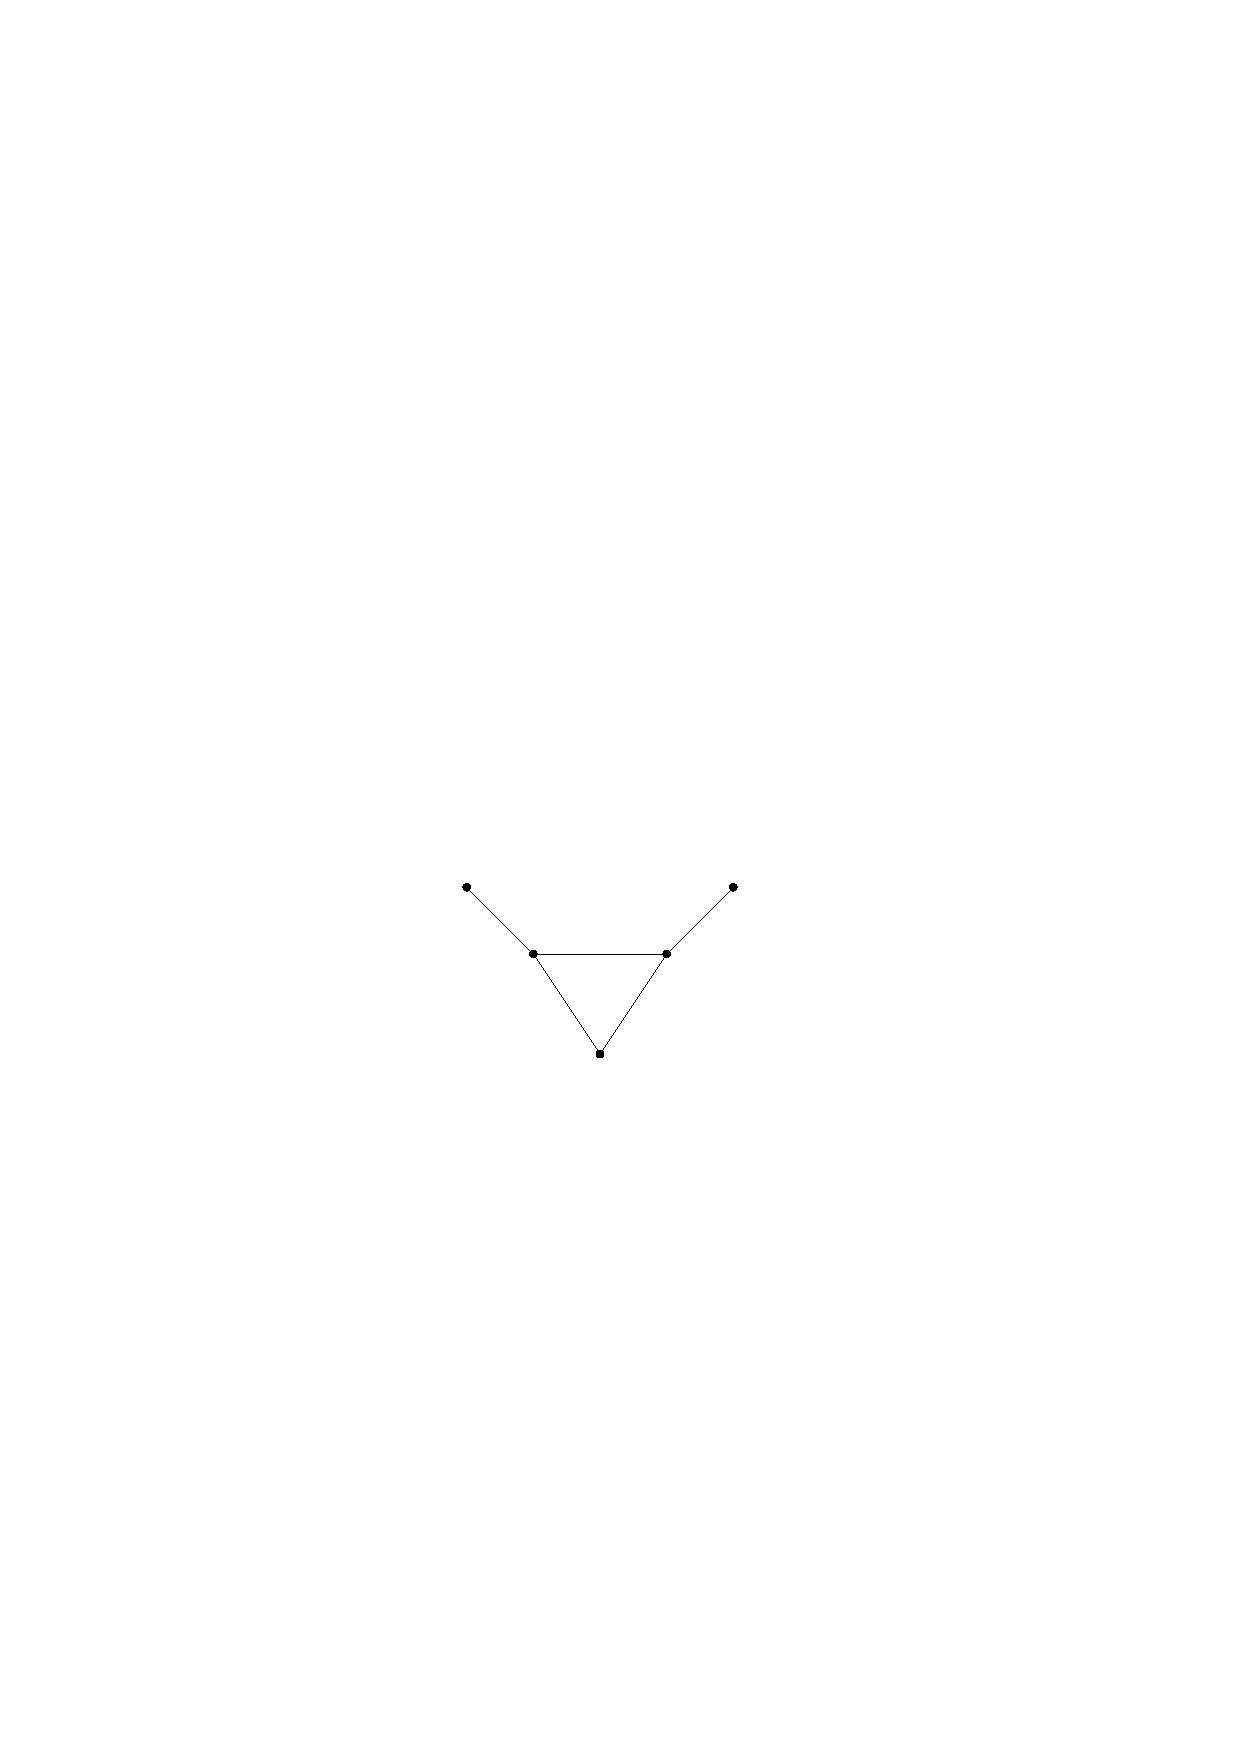
\includegraphics{Images/BullGraph.pdf}
\end{center}

\begin{Theorem}\label{thm:SCOrder}
The order of any self-complementary graph is $4k$ or $4k + 1$, for some non-negative integer $k$.
\end{Theorem}

\begin{proof}
Let $G$ be a self-complementary graph of order $n$ and size $m$. Then the size of $\overline G$ is $\binom n 2 - m$. Since $G \cong \overline G$, $m = \binom n 2 - m$, which implies that $m = \frac 1 2 \binom n 2 = \frac {n(n - 1)}{4}$. As $m$ is an integer, this implies that $4$ divides $n(n - 1)$, which in turn implies that either one of $n$ and $n - 1$ is divisible by $4$, or both $n$ and $n - 1$ are even. Since the latter is not possible, it follows that $n = 4k$ or $n - 1 = 4k$, i.e., $n = 4k$ or $4k + 1$ for some integer $k$.
\end{proof}


From \cref{thm:GorGCompConn}, we know that a graph and its complement cannot both be disconnected. Thus, if $G$ is a disconnected graph, then $\overline G$ must be connected, and therefore it cannot be isomorphic to $G$. This implies that a self-complementary graph is necessarily connected.

\begin{Corollary}\label{cor:SCConn}
Every self-complementary graph is connected. \qed
\end{Corollary}

Similarly, from \cref{thm:Diam>=3}, we obtain the following corollary about the diameter of self-complementary graphs.

\begin{Corollary}
Every non-trivial self-complementary graph has diameter $2$ or $3$.
\end{Corollary}

\begin{proof}
Consider a non-trivial, self-complementary graph $G$, and suppose that it has diameter strictly greater than $3$. Then, by \cref{thm:Diam>=3}, $\diam \overline G \le 3$, which implies that $\diam \overline G \ne \diam G$, a contradiction, since $G \cong \overline G$. Hence, $\diam G \le 3$. On the other hand, a non-trivial graph cannot have diameter $0$, hence $\diam G \ge 1$. But if $\diam G = 1$, then $G$ is a non-trivial complete graph, whose complement is a totally disconnected graph, which is again impossible. Hence, $\diam G = 2$ or $3$.
\end{proof}

\begin{Exercise}
If $G$ is a regular self-complementary graph of order $n$, show that $n = 4k + 1$, for some integer $k$, and $\diam G = 2$.
\end{Exercise}

\begin{Exercise}
Let $G$ be a self-complementary graph, and let $H$ be the graph obtained by taking the disjoint union of $H$ and $P_4$, and making every vertex of $H$ adjacent to the two non-pendant vertices of this $P_4$. Then show that $H$ is also self-complementary. What is the graph $H$ obtained in this manner if $G = K_1$?
\end{Exercise}

\begin{Exercise}
Construct a self-complementary graph of order $9$.
\end{Exercise}

\begin{Exercise}
Show that for each positive integer $n$ of the form $4k$ or $4k + 1$, where $k$ is an integer, there exists at least one self-complementary graph of order $n$.
\end{Exercise}

\section{Bipartite Graphs}\label{sec:Bipartite}

A graph $G = (V, E)$ is \newterm{bipartite} if its vertex set $V$ can be partitioned into two subsets $V_1$ and $V_2$ such that no two vertices in $V_i$ are adjacent, for $i = 1, 2$. That is, there exist two non-empty, disjoint subsets $V_1, V_2 \subseteq V$ such that $V_1 \cup V_2 = V$, and every edge of $G$ (if any) joins a vertex in $V_1$ with a vertex in $V_2$. Then we say that $(V_1, V_2)$ is a \newterm{bipartition} of $G$.

The following theorem characterises bipartite graphs in terms of its cycles. A cycle is \newterm{even} if its length is even and \newterm{odd} if its length is odd.

\begin{Theorem}
A graph is bipartite if and only if it contains no odd cycles.
\end{Theorem}

\begin{proof}
First, suppose that $G$ is a bipartite graph with bipartition $(V_1, V_2)$, and let $v_1, v_2, \ldots, v_k$ be a cycle of length $k$ in $G$. Without loss of generality, suppose that $v_1 \in V_1$. Then, since $v_2 \sim v_1$, $v_2 \in V_2$, which in turn implies that $v_3 \in V_1$, as $v_2 \sim v_3$. Proceeding similarly, we see $v_i \in V_1$ if $i$ is odd and $v_i \in V_2$ if $i$ is even. But $v_k \sim v_1$ and $v_1 \in V_1$ implies that $v_k \in V_2$. Therefore, $k$ (the length of the cycle) is even.

Conversely, suppose $G$ is a graph that has no odd cycles. Without loss of generality, assume that $G$ is connected -- otherwise, apply the argument to each component. Let $v$ be any vertex of $G$. Define subsets $V_1$ and $V_2$ of $V(G)$ as follows:
\begin{align*}
    V_1 = \qty{\, u \in V \mid d(u, v)\ \text{is even} \,} \\
    V_2 = \qty{\, u \in V \mid d(u, v)\ \text{is odd} \,}.
\end{align*}
We claim that $(V_1, V_2)$ is a bipartition of $G$.

Suppose not, and let $x$ and $y$ be adjacent vertices of $G$, both belonging to $V_i$ for $i = 1$ or $2$. Let $P$ and $Q$ be shortest paths from $v$ to $x$ and $y$ respectively. Let $w$ be the last vertex common to both $P$ and $Q$ when traversing $P$ from $v$ to $x$. Then the portion of $P$ from $w$ to $x$, the edge $(x, y)$, and the portion of $Q$ from $y$ to $w$ forms a cycle in $G$, having length, say $l$, given by
\begin{align*}
l & = d(w, x) + d(w, y) + 1 \\
& = [d(v, x) - d(v, w)] + [d(v, y) - d(v, w)] + 1 \\
& = d(v, x) + d(v, y) - 2 d(v, w) + 1.
\end{align*}
If $x, y \in V_1$, then both $d(v, x)$ and $d(v, y)$ are even, and if $x, y \in V_2$, then both these numbers are odd. In either case, $d(v, x) + d(v, y)$ is even, and hence $l$ is odd, which is a contradiction. Hence, $(V_1, V_2)$ is a bipartition of $G$ as claimed.
\end{proof}

\section{Trees}\label{sec:Trees}

A \newterm{tree} is a connected, acyclic graph. There are several well known characterisations or alternative definitions of trees. We take the given definition as the basic one and prove its equivalence to some others.

\begin{Theorem}\label{thm:UniPath}
A graph $T$ is a tree if and only if there is a unique path joining every two vertices of $T$.
\end{Theorem}
\begin{proof}
First, suppose that $T$ is a tree, and let $u$ and $v$ be vertices of $T$. Since $T$ is connected, there is a path, say $P_1$, joining $u$ and $v$. Now we must show that this path is unique. Assume to the contrary that there exists another path $P_2$ from $u$ to $v$. When traversing $P_1$ from $u$ to $v$, let $w$ be the first vertex that is present on $P_1$ but not $P_2$. Let $x$ be the vertex on $P_1$ preceding $w$, and note that $x$ is on $P_2$ as well. Let $y$ be the next vertex common to both $P_1$ and $P_2$ when traversing $P_1$ from $x$ to $v$. Then the portion of $P_1$ from $x$ to $y$ together with the portion of $P_2$ from $y$ to $x$ forms a cycle in the tree $T$, which is a contradiction. Thus, $P_1$ is the unique path joining $u$ and $v$.

Conversely, suppose that $T$ is a graph in which there is a unique path joining any two vertices. Clearly, $T$ is connected. To show that $T$ is acyclic, suppose that $v_1, v_2, \ldots, v_n$ is a cycle in $T$. Then we get two different paths joining $v_1$ and $v_n$, namely the path $v_1, v_2, \ldots, v_n$ and the path $v_1, v_n$ (since $v_1 \sim v_n$ in the cycle). This contradicts our assumption. Thus, $T$ must be acyclic and hence is a tree.
\end{proof}

The next two results show that the size of a tree is always one less than its order, and that conversely, this property together with either connectedness or acyclicity implies that the graph is a tree.
\begin{Theorem}\label{thm:Conn;p=q+1}
A $(p, q)$-graph $T$ is a tree if and only if it is connected and $p = q + 1$.
\end{Theorem}
\begin{proof}
Let $T$ be a tree with $p$ vertices and $q$ edges. Then $T$ is connected. We prove that $p = q + 1$ by induction. This is clearly true when $p = 1$. Assume it to be true for all trees of order less than $p$. Now in $T$, we know that every two vertices are joined by a unique path. Thus, if $e$ is any edge of $T$, then the graph $T - \{e\}$ obtained by deleting $e$ has exactly two components, say $T_1$ and $T_2$. Each one is a tree, since it is connected and acyclic. Let $T_i$ have $p_i$ vertices and $q_i$ edges, $i = 1, 2$. Then by the hypothesis, $p_i = q_i + 1$ (since $p_i < p$). But $p = p_1 + p_2$ and $q = q_1 + q_2 + 1$ (since the size of $T - \{e\}$ is one less than that of $T$). Thus, $p = q_1 + q_2 + 2 = q + 1$.

For the converse, suppose that $T$ is a connected $(p,q)$-graph with $p = q + 1$. We must show that is acyclic. Suppose to the contrary that $T$ has a cycle $C$ with $k$ vertices. Then $C$ has $k$ edges as well. Since $T$ is connected, there is a path from every vertex not on $C$ to some vertex of $C$. The shortest path from each vertex $v$ not on $C$ to a vertex on $C$ has a unique edge incident with $v$, which is not part of $C$. Since there are $p - k$ vertices in $T$ not on $C$, there are $p - k$ such edges. Thus $q \ge (p - k) + k = p$, which contradicts our assumption that $p = q + 1$. Thus, $T$ must be acyclic.
\end{proof}

In the following theorem, the proof of the direct part is identical to that of Theorem~\ref{thm:Conn;p=q+1}, except for the assertion being about acyclicity rather than connectedness. The proof of the converse part is entirely different.
\begin{Theorem}\label{thm:Acyc;p=q+1}
A $(p,q)$-graph $T$ is a tree if and only if it is acyclic and $p = q + 1$.
\end{Theorem}
\begin{proof}
Let $T$ be a tree with $p$ vertices and $q$ edges. Then $T$ is acyclic. We prove that $p = q + 1$ by induction. This is clearly true when $p = 1$. Assume it to be true for all trees of order less than $p$. Now in $T$, we know that every two vertices are joined by a unique path. Thus, if $e$ is any edge of $T$, then the graph $T - \{e\}$ obtained by deleting $e$ has exactly two components, say $T_1$ and $T_2$. Each one is a tree, since it is connected and acyclic. Let $T_i$ have $p_i$ vertices and $q_i$ edges, $i = 1, 2$. Then by the hypothesis, $p_i = q_i + 1$ (since $p_i < p$). But $p = p_1 + p_2$ and $q = q_1 + q_2 + 1$ (since the size of $T - \{e\}$ is one less than that of $T$). Thus, $p = q_1 + q_2 + 2 = q + 1$.

Conversely, suppose that $T$ is an acyclic $(p,q)$-graph with $p = q + 1$. To show that $T$ is connected, we need to prove that it is connected -- i.e., it has only one component. Let $T$ have $k$ components $T_1, \ldots, T_k$. Each one is acyclic, and being connected, is a tree. Thus from the first part of the theorem, we know that if $p_i$ and $q_i$ are respectively the order and size of the component $T_i$, $p_i = q_i + 1$. Now $p = p_1 + \cdots p_k = (q_1 + 1) + \cdots (q_k + 1) = q + k$. But we know that $p = q + 1$. Therefore, $k = 1$. Thus, $T$ is a tree.
\end{proof}

\begin{Exercise}
A \newterm{pendant vertex} of a graph is a vertex of degree $1$. Prove that every non-trivial tree contains at least two pendant vertices.\\
    \hint{Observe that a non-trivial tree cannot have a vertex of degree zero. Use Handshaking Lemma and assume every degree is at least $2$ to get a contradiction.}
\end{Exercise}

\begin{Exercise}
The \newterm{centre} of a graph $G$ is the set of all vertices of $G$ with minimum eccentricity -- i.e., the set of all vertices $v$ of $G$ with $\ecc v = \rad v$. Show that every tree has a centre consisting of either exactly one vertex or exactly two adjacent vertices.\\
\hint{Observe that deleting all pendant vertices of a tree results in a new tree with the same centre.}
\end{Exercise}

\begin{Solution*}
Let $T$ be a tree on $n$ vertices. We prove the result by induction on $n$.

If $n = 1$ or $2$, the result obviously holds. Suppose, for the sake of induction, that the result holds for all trees of order less than $n$.

Consider $T$, of order $n \ge 3$. Then $T$ has at least two pendant vertices. Let $T'$ be the tree (of order less than $n$) obtained by deleting all the pendant vertices of $T$.

Then the vertices of $T'$ have eccentricities exactly one less than their eccentricities in $T$, and therefore, $T$ and $T'$ have the same centre. Hence, the result follows by induction.
\end{Solution*}

\begin{Exercise}
If $G$ and $H$ are two trees of orders $n$ and $m$ respectively, what is the size of $G \times H$?
\end{Exercise}

\section{Blocks}\label{sec:Blocks}
A \newterm{cutvertex} of a graph is a vertex whose removal increases the number of components, i.e., a vertex $v$ of $G$ such that $G - v$ has more components than $G$. If $G$ is connected, we can equivalently say that $v$ is a cutvertex if $G - v$ is disconnected. Similarly, a \newterm{cutedge} or \newterm{bridge} of a graph whose removal increases the number of components. A \newterm{nonseparable} graph is a connected, non-trivial graph with no cutvertices. A maximal nonseparable subgraph of a graph is a \newterm{block} of the graph. A nonseparable graph is itself said to be a block as well.

\begin{Example}\label{ex:Blocks}
The graph shown below has $6$ blocks and $3$ cutvertices ($v_1$, $v_2$, $v_3$).
\begin{center}
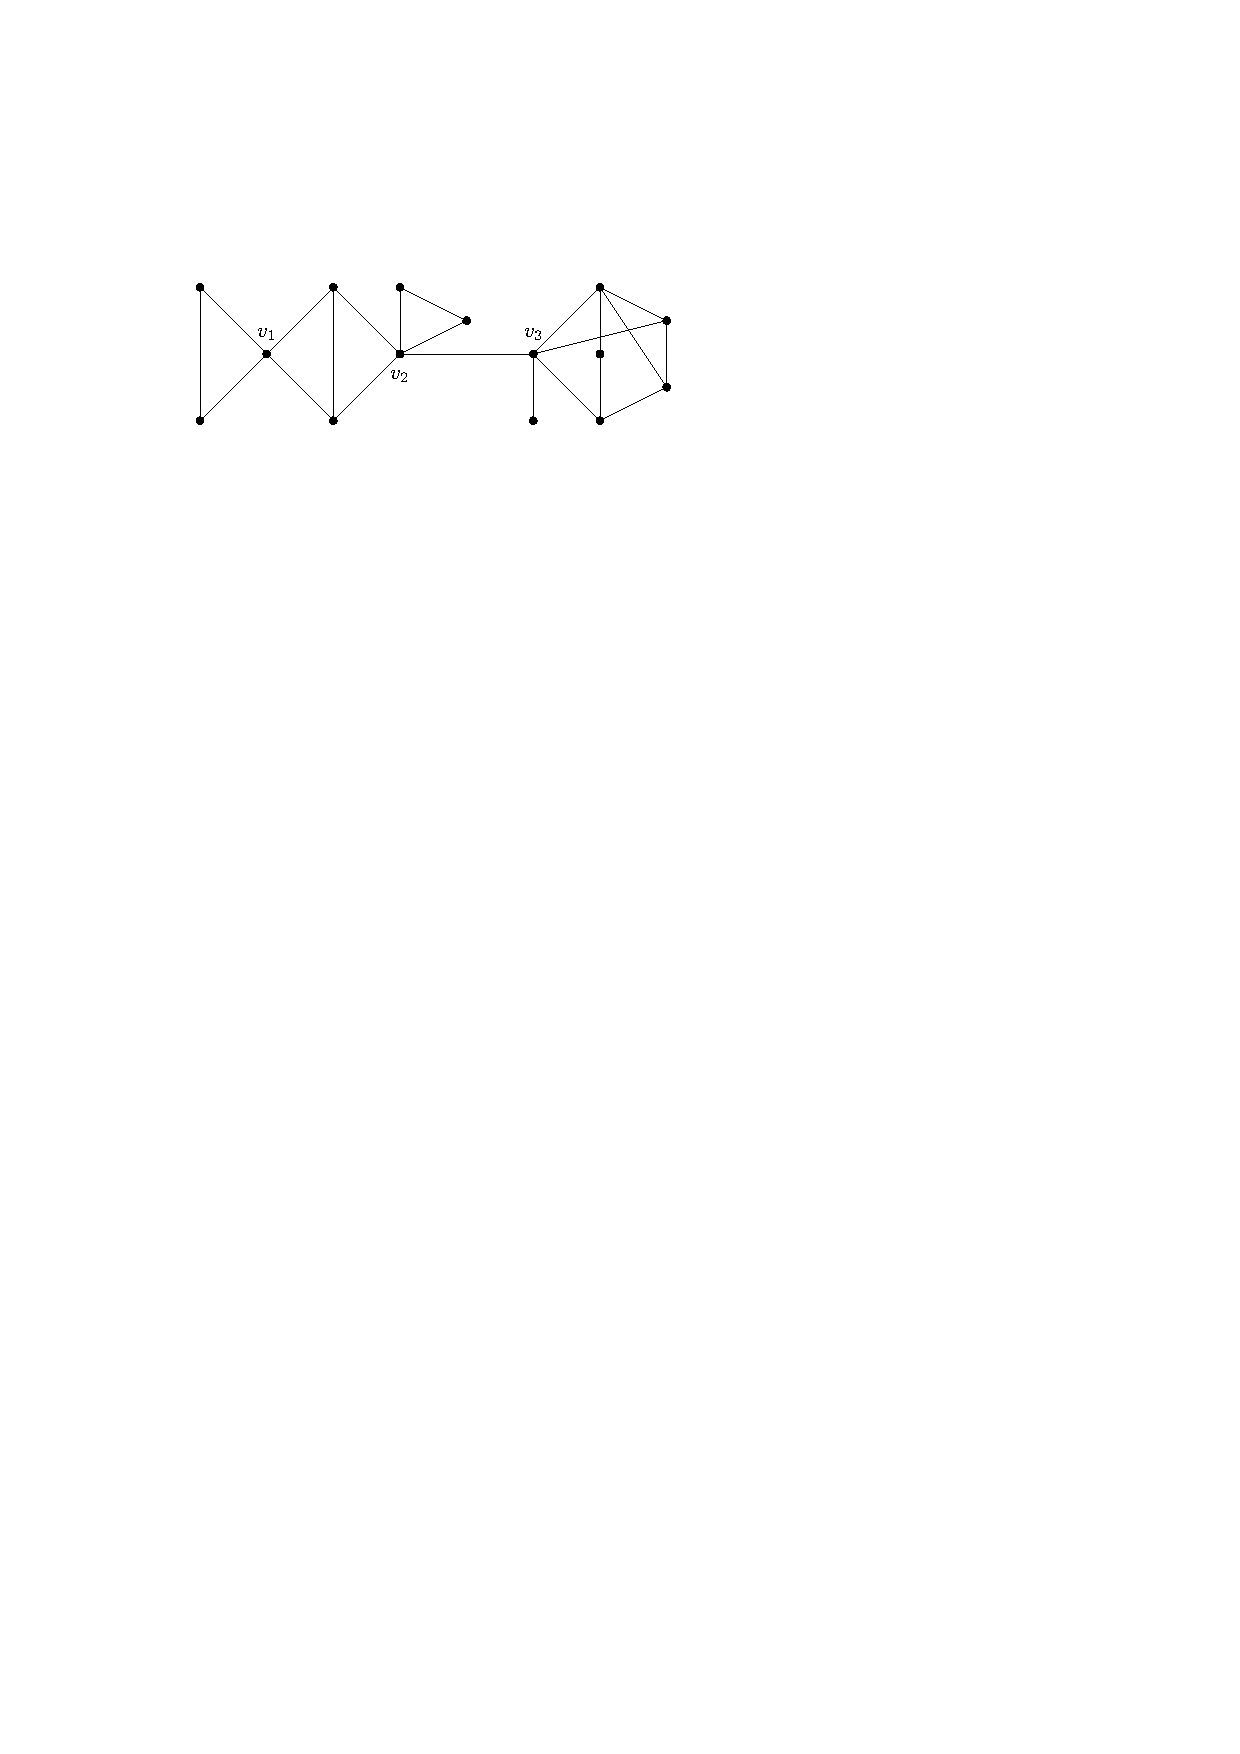
\includegraphics{Images/6BlockGraph2.pdf}
\end{center}
The $6$ blocks of this graph are shown below.
\begin{center}
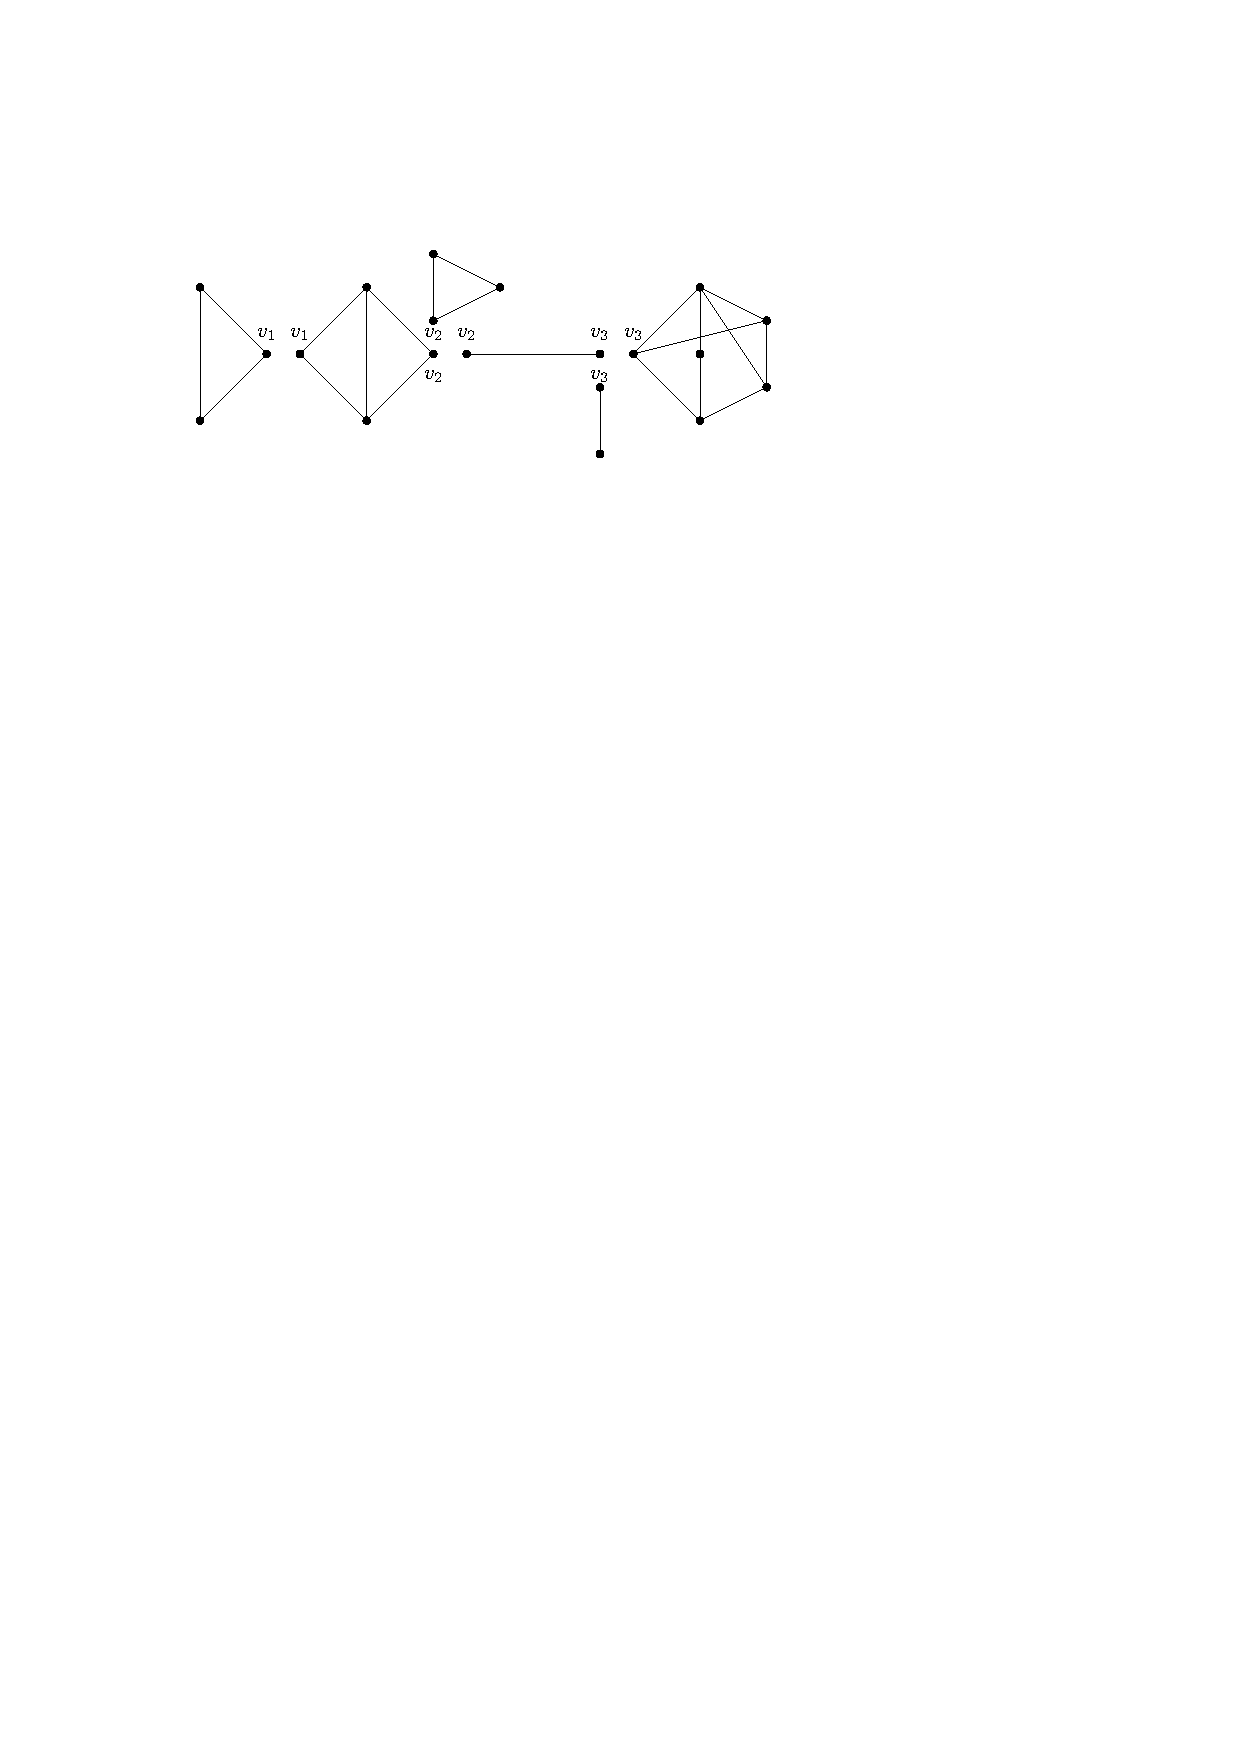
\includegraphics{Images/6BlockGraph2-Blocks.pdf}
\end{center}
\end{Example}

\begin{Theorem}\label{thm:CutverChar}
If $G$ is a connected graph, and $v$ is any vertex of $G$, then the following are equivalent:
\begin{enumerate}[label=(\roman*)]
\item\label{it:CutverChar1} $v$ is a cutvertex of $G$.
\item\label{it:CutverChar2} There exist vertices $u$ and $w$ of $G$, distinct from $v$, such that every $u$-$w$ path passes through $v$.
\item\label{it:CutverChar3} There exists a partition of $V(G) - v$ into two non-empty subsets $U$ and $W$ such that for all $u \in U$ and $w \in W$, every $u$-$w$ path passes through $v$.
\end{enumerate}
\end{Theorem}

\begin{proof}
\cref{it:CutverChar1} $\implies $ \cref{it:CutverChar3}. Since $v$ is a cutvertex, the graph $G - v$ is disconnected, i.e., it has two or more components. Let $U$ be the set of all the vertices in any one of the components, and let $W$ be the set of all the remaining vertices of $G - v$. Clearly, $\{U, W\}$ is a partition of $V(G) - v$. Now, if $u \in U$ and $w \in W$, then $u$ and $w$ are in different components of $G - v$, which implies that any path from $u$ to $w$ must pass through $v$.

\noindent \cref{it:CutverChar3} $\implies$ \cref{it:CutverChar2} is obvious as the latter is a special case of the former.

\noindent \cref{it:CutverChar2} $\implies$ \cref{it:CutverChar1}. Consider the graph $G - v$. As every $u$-$w$ path passes through $v$, none of them is present in $G - v$, and therefore $G - v$ is disconnected. Hence, $v$ is a cutvertex of $G$.
\end{proof}

\section{Line Graphs}\label{sec:LineGraphs}

Let $G$ be a graph with at least one edge. The \newterm{line graph} of $G$ is the graph $L(G)$ whose vertex set is the edge set of $G$, in which two vertices $e$ and $f$ are adjacent if the edges $e$ and $f$ of $G$ are adjacent.

\begin{Example}\label{ex:LineGrpahs}
\cref{fig:LineGraphs} shows a graph $G$ with eight edges and and its line graph $L(G)$.
\begin{figure}[!htbp]
\centering
\subcaptionbox{$G$}{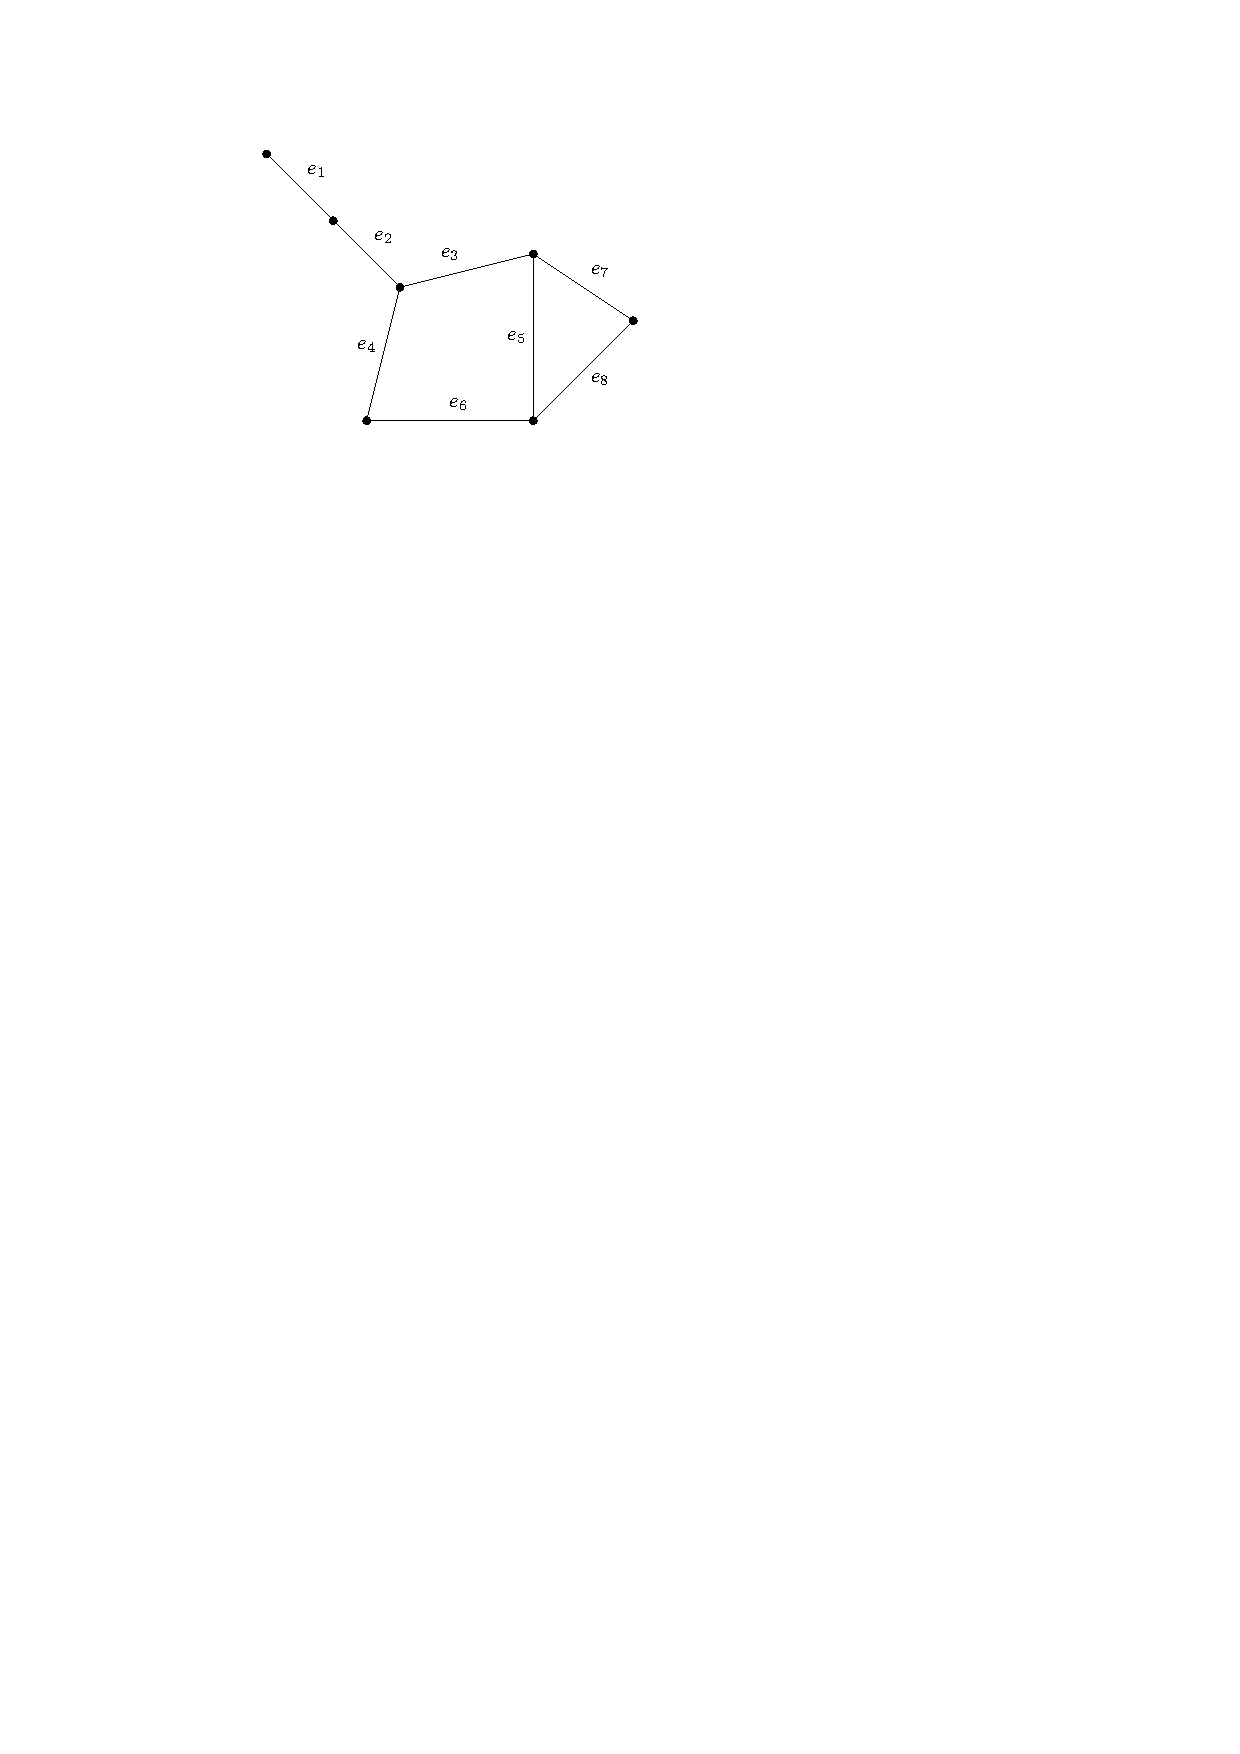
\includegraphics{Images/GNM(7,8).pdf}} \hspace{5em}
\subcaptionbox{$L(G)$}{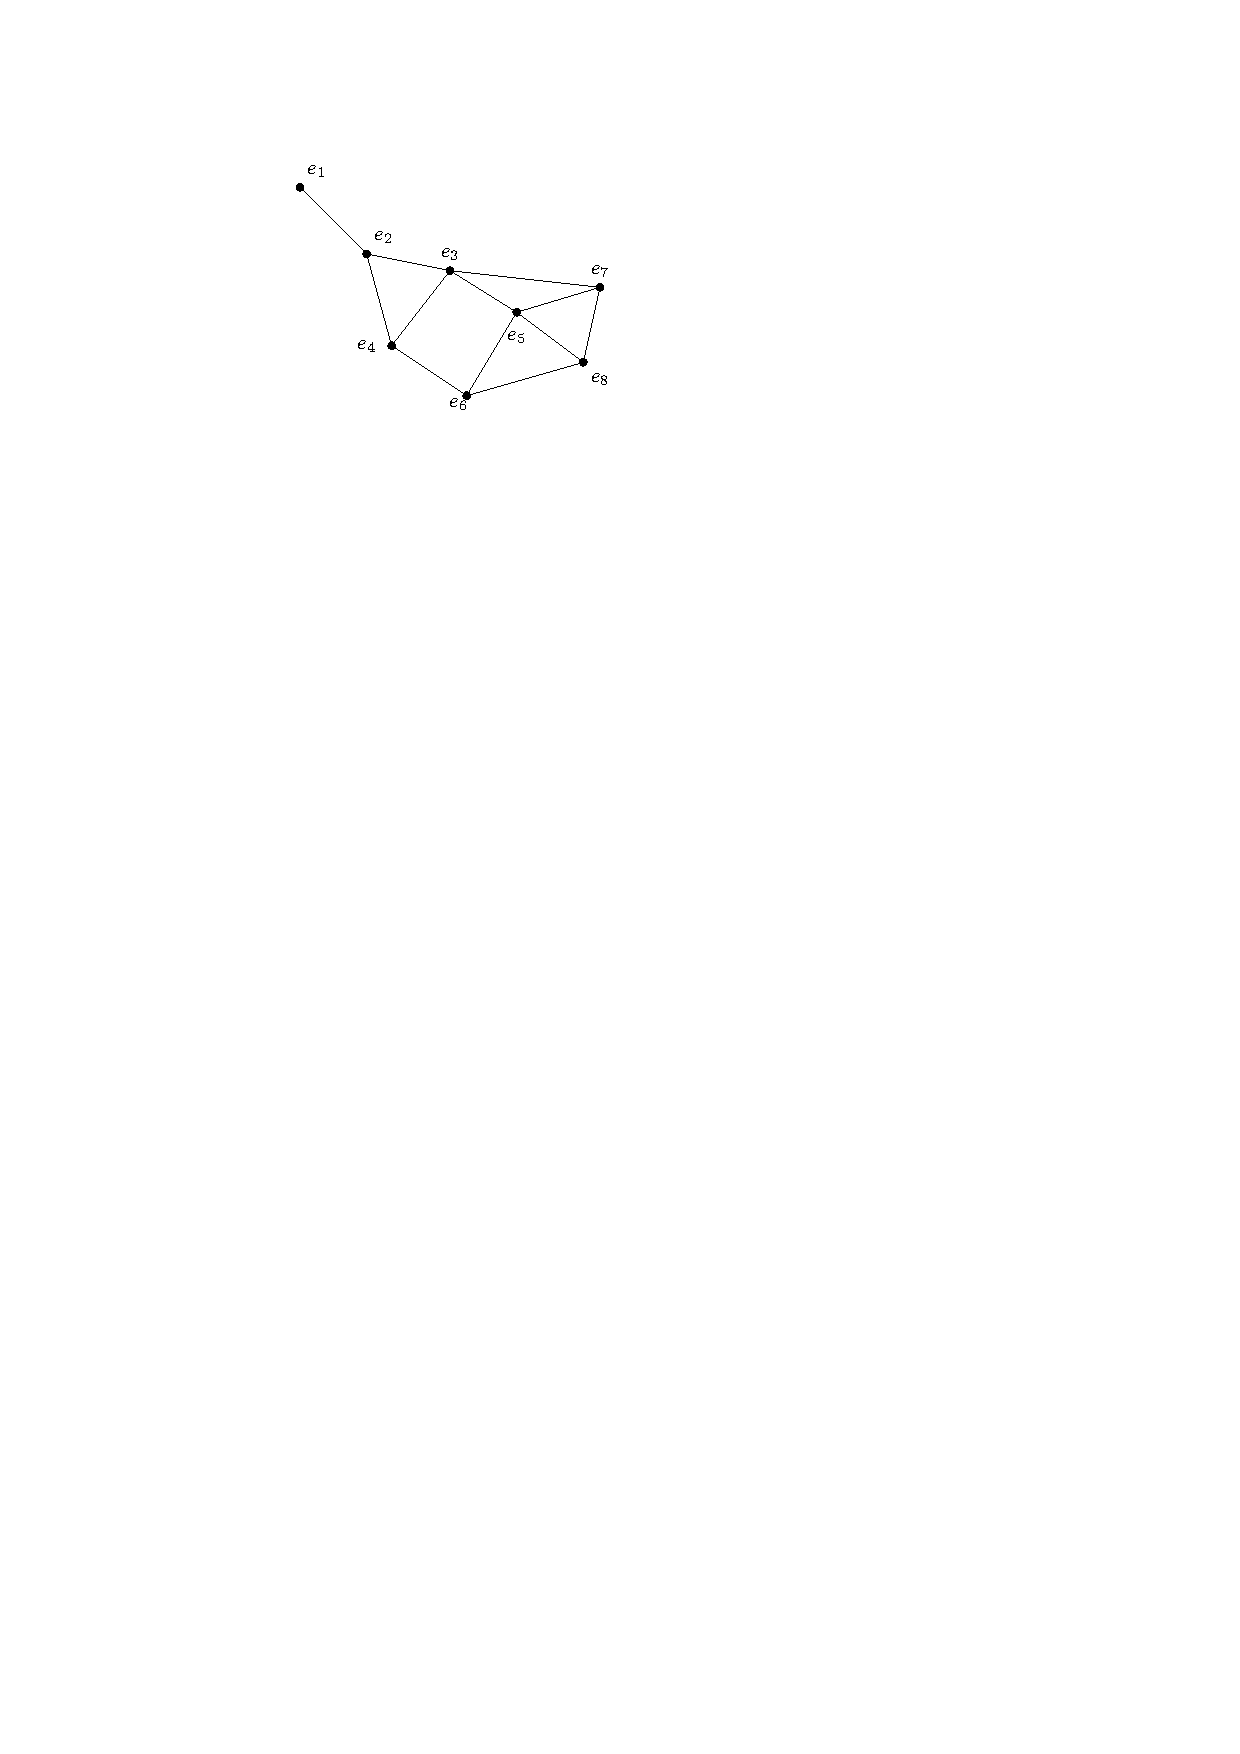
\includegraphics{Images/L(GNM(7,8)).pdf}}
\caption{A graph and its line graph}\label{fig:LineGraphs}
\end{figure}
\end{Example}

If $u$ and $v$ are edges joined by an edge $e$ in $G$, then in $L(G)$, the vertex $e$ will be adjacent to all the vertices corresponding to the edges of $G$ other than $e$ that are incident with $u$ and $v$ (see \cref{fig:L(G)Neighbourhood}). Thus, $\deg_{L(G)} e = \deg_G u + \deg_G v - 2$.
\begin{figure}[!htbp]
\centering
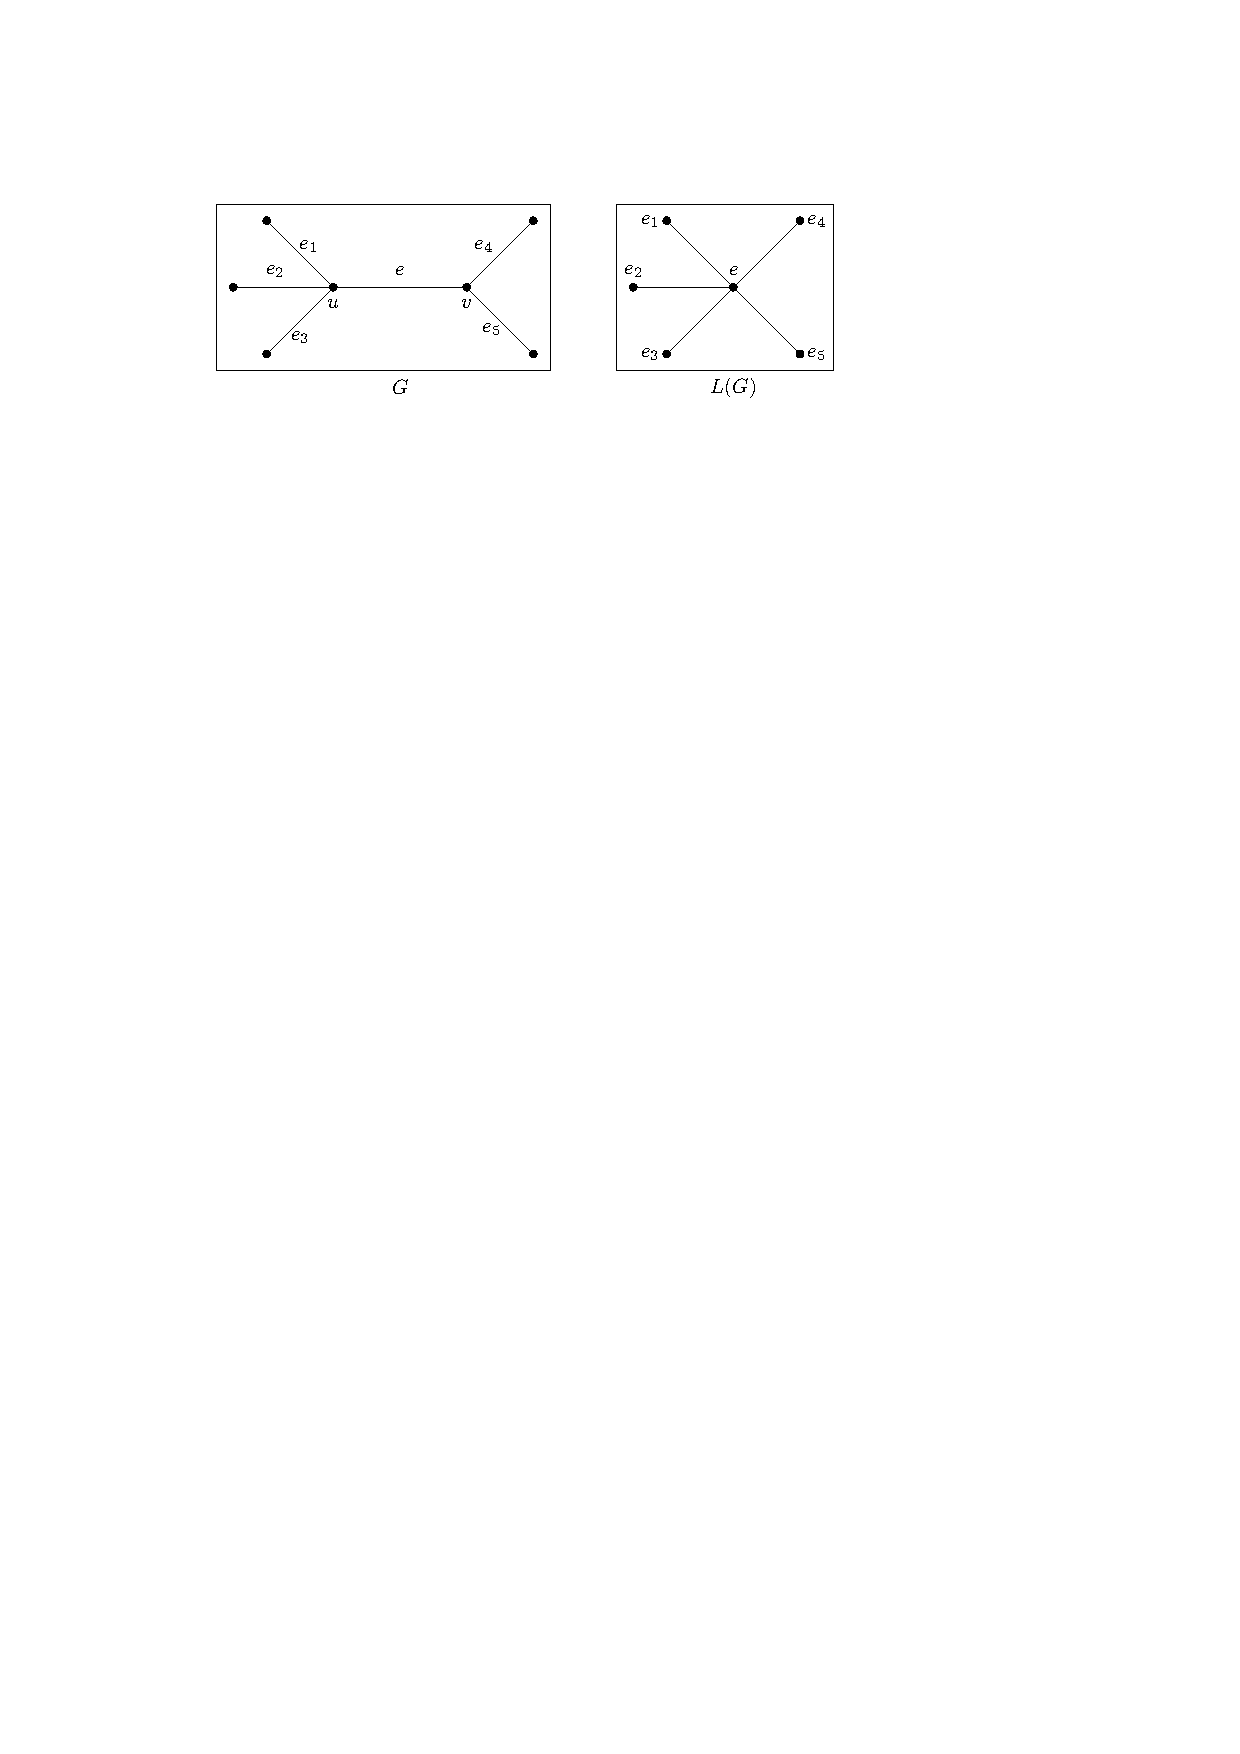
\includegraphics{Images/L(G)Neighbourhood.pdf}
\caption{Neighbourhood of a vertex in $L(G)$}
\label{fig:L(G)Neighbourhood}
\end{figure}

\begin{Theorem}
For any graph $G$ of size $m \ge 1$, its line graph $L(G)$ has order $m$ size $\displaystyle\sum_{v \in V(G)} \binom{\deg_G v}{2}$.
\end{Theorem}

\begin{proof}
By definition, the vertices of $L(G)$ are the edges of $G$, and hence the order of $L(G)$ is the size of $G$, $m$.

Now, let $e = uv$ be an edge of $G$. In $L(G)$, $e$ is a vertex, and it is adjacent to another vertex $f$ if and only if $f$ is an edge of $G$ and is adjacent to $e$, i.e. $f$ is an edge of $G$ incident with one of the end vertices of $e$, namely $u$ and $v$. Thus, the degree of the vertex $e$ of $L(G)$ is equal to the total number of edges that are incident with either $u$ or $v$ in $G$, except for the edge $e$ itself.

Clearly, $u$ is incident with to $\deg_G u - 1$ edges other than $e$, and $v$ is incident with $\deg_G v - 1$ edges other than $e$. Thus, the degree of $e$ in $L(G)$ is $\deg_G u  - 1 + \deg_G v - 1$.

By Handshaking Lemma, the size of $L(G)$ is half the sum of its vertex degrees, which is
\begin{equation*}
	\frac 1 2 \sum_{uv \in E(G)} (\deg_G u - 1 + \deg_G v - 1).
\end{equation*}
As the summation is over the edges of $G$, each vertex $v$ of $G$ appears exactly $\deg v$ times in the above summation, which can therefore be written as
\begin{equation*}
	\pushQED{\qed}
	\frac 1 2 \sum_{v \in V(G)} (\deg_G v)(\deg_G v - 1) = \sum_{v \in V(G)} \binom{\deg_G v}{2}.\qedhere
\end{equation*}
\end{proof}

\section{Adjacency Matrices}\label{sec:AdjMat}

The \newterm{adjacency matrix} of a graph $G$ of order $n$, with vertex set $V = \{v_1, \ldots, v_n\}$, is the $n \times n$ matrix $A = A(G)$ whose $(i,j)$-entry is
\begin{equation*}
a_{ij} = \begin{cases}
1, & v_i \sim v_j \\
0, & v_i \nsim v_j.
\end{cases}
\end{equation*}

\begin{Example}\label{ex:GNM(6-11)AdjMat}
The adjacency matrix of the graph
\begin{center}
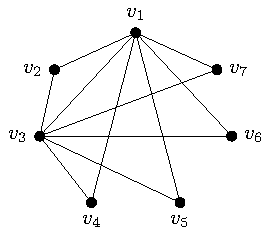
\includegraphics{Images/GNM(6,11).pdf}
\end{center}
is
\begin{equation*}
A = \begin{bmatrix}
0 & 1 & 1 & 1 & 1 & 1 & 1 \\
1 & 0 & 1 & 0 & 0 & 0 & 0 \\
1 & 1 & 0 & 1 & 1 & 1 & 1 \\
1 & 0 & 1 & 0 & 0 & 0 & 0 \\
1 & 0 & 1 & 0 & 0 & 0 & 0 \\
1 & 0 & 1 & 0 & 0 & 0 & 0 \\
1 & 0 & 1 & 0 & 0 & 0 & 0
\end{bmatrix}.
\end{equation*}
\end{Example}

Observe that, as the graphs we discuss are simple graphs and therefore have no self-loops on vertices, no vertex is adjacent to itself -- i.e., $a_{ii} = 0$ for all $i = 1, \ldots, n$. Also, since the graphs are undirected, $v_i \sim v_j$ if and only if $v_j \sim v_i$ -- i.e., $a_{ij} = a_{ji}$. Thus, we have the following observation.

\begin{Observation}
The adjacency matrix of a (simple, undirected) graph is a symmetric, zero-diagonal, $0$-$1$ matrix.
\end{Observation}

In the $i$\th row of the adjacency matrix, for each $j$, the $j$\th entry is $1$ if $v_j$ is adjacent to $v_i$, and $0$ otherwise. That is, the number of $1$s in the $i$\th row is the number of vertices adjacent to $v_i$, or in other words, the degree of $v_i$. Thus, the row sums of $A$ are the vertex degrees. Observe that $A \mathbbm 1$ is the vector of row sums, where $\mathbbm 1$ is the vector (of suitable size) with all entries equal to $1$. For instance, with the matrix $A$ given in \cref{ex:GNM(6-11)AdjMat},
\begin{equation*}
A = \begin{bmatrix}
0 & 1 & 1 & 1 & 1 & 1 & 1 \\
1 & 0 & 1 & 0 & 0 & 0 & 0 \\
1 & 1 & 0 & 1 & 1 & 1 & 1 \\
1 & 0 & 1 & 0 & 0 & 0 & 0 \\
1 & 0 & 1 & 0 & 0 & 0 & 0 \\
1 & 0 & 1 & 0 & 0 & 0 & 0 \\
1 & 0 & 1 & 0 & 0 & 0 & 0
\end{bmatrix}
\begin{bmatrix}
1 \\ 1 \\ 1 \\ 1 \\ 1 \\ 1 \\ 1
\end{bmatrix} =
\begin{bmatrix}
6 \\ 2 \\ 6 \\ 2 \\ 2 \\ 2 \\ 2
\end{bmatrix}.
\end{equation*}
From the Handshaking Lemma and the preceding observation, it follows that the sum of all entries of $A$ is twice the number of edges of the graph.

\begin{Exercise}\label{exer:A2ij}
Show that the $(i,j)$-entry of $A^2$ is the number of walks of length $2$ from $v_i$ to $v_j$. Hence show that $\trace(A^2) = 2|E(G)|$.\\
\hint{Recall that if $A$ is any $n \times n$ matrix, then the $(i,j)$-entry of $A^2$ is $\sum_{k=1}^{n} a_{ik}a_{kj}$. As $A$ is a $0$-$1$ matrix, each term in this summation is $1$ or $0$, with the former if and only if $a_{ik} = a_{kj} = 1$. What does this imply about the vertices $v_i$, $v_k$, and $v_j$? Then, as $k$ varies from $1$ to $n$, what does the value of the sum imply about $v_i$ and $v_j$?}
\end{Exercise}

The following result (which generalises the statement in \cref{exer:A2ij}) shows that the adjacency matrix can be used to obtain certain information about walks in the graph.

\begin{Theorem}
Let $A$ be the adjacency matrix of a graph $G$ with vertex set $\{v_1, \ldots, v_n\}$. Then the $(i,j)$-entry of $A^m$, for any positive integer $m$, is the number of walks of length $m$ from $v_i$ to $v_j$.
\end{Theorem}

\begin{proof}
We prove the result by induction on $m$. For $m = 1$, the $(i,j)$-entry of $A^1 = A$ is $a_{ij}$, which is $1$ if and only if $v_i$ is adjacent to $v_j$, i.e., if and only if there is a walk of length $1$ (namely, an edge) from $v_i$ to $v_j$. Thus, the result holds for $m = 1$.

Now suppose, for the sake of induction, that the result holds for some $m \ge 1$, and consider $A^{m + 1}$. The $(i,j)$-entry of $A^{m + 1}$ is
\begin{equation*}
(A^{m + 1})_{ij} = \sum_{k = 1}^{n} (A^m)_{ik} a_{kj}.
\end{equation*}
First, note that $a_{kj} = 1$ if and only if $v_k \sim v_j$. Therefore, the above sum is equal to the sum of all $(A^m)_{ik}$ where $v_k \sim v_j$. Now, by the induction hypothesis, $(A^m)_{ik}$ is the number of walks of length $m$ from $v_i$ to $v_k$. If $v_j$ is adjacent to $v_j$, then each walk of length $m$ from $v_i$ to $v_k$, together with the edge from $v_j$ to $v_j$, forms a walk of length $m + 1$ from $v_i$ to $v_j$. Thus, for each $k$ such that $v_k \sim v_j$, $(A^m)_{ik} a_{kj} = (A^m)_{ik}$ is the number of walks of length $m + 1$ from $v_i$ to $v_j$ that pass through $k$. Summing over all $k$, this gives the total number of walks of length $m + 1$ from $v_i$ to $v_j$. Hence the result follows by induction.
\end{proof}

\begin{Theorem}
Let $A$ be the adjacency matrix of a graph $G$ with vertex set $\{v_1, \ldots, v_n\}$. Then
\begin{enumerate}[label=(\roman*)]
\item $\tr(A^2) = 2 |E(G)|$
\item $\tr(A^3) = 6 c_3(G)$
\end{enumerate}
where $c_3(G)$ denotes the number of triangles in $G$.
\end{Theorem}

\begin{proof}
We know that $(A^m)_{ij}$ is the number of walks of length $m$ from $v_i$ to $v_j$.
\begin{enumerate}[label=(\roman*)]
\item Hence, the $i$\nth diagonal entry of $A^2$, viz. $(A^2)_{ii}$, is the number of walks of length $2$ from $v_i$ to itself. Any walk of length $2$ from $v_i$ to itself is of the form $v_i v_j v_i$, where $v_j$ is a vertex adjacent to $v_i$. Thus, the number of such walks is equal to the number of vertices adjacent to $v_i$, i.e. $\deg v_i$. Hence, $\tr(A^2) = \sum_{i=1}^n \deg v_i = 2|E(G)|$, by Handshaking Lemma.

\item Similarly, $(A^3)_{ii}$ is the number of walks of length $3$ from $v_i$ to itself. Any such walk is of the form $v_i v_j v_k v_i$, which implies that $v_i$, $v_j$, and $v_k$ form a triangle in $G$. Moreover, each such triangle corresponds to two distinct walks from $v_i$ to itself, when traversed in the two opposite directions. Thus, $(A^3)_{ii}$ is twice the number of triangles having $v_i$ as one of its vertices. Therefore, $\tr(A^3)$ is $6 c_3(G)$, since each triangle contains three vertices, each of which counts the triangle twice in the sum $\tr(A^3)$.
\end{enumerate}
\end{proof}

\section{Incidence Matrices}\label{sec:IncMat}

Consider an $(n, m)$-graph $G$ having vertex set $\{v_1, \ldots, v_n\}$ and edge set $\{e_1, \ldots, e_m\}$. The \newterm{incidence matrix} of $G$ is the $n \times m$ matrix $B = B(G)$ whose $(i, j)$-entry is $1$ if the vertex $v_i$ is incident with the edge $e_i$, and $0$ otherwise.

\begin{Example}\label{ex:GNM(6-8)AdjMat}
The incidence matrix of the graph
\begin{center}
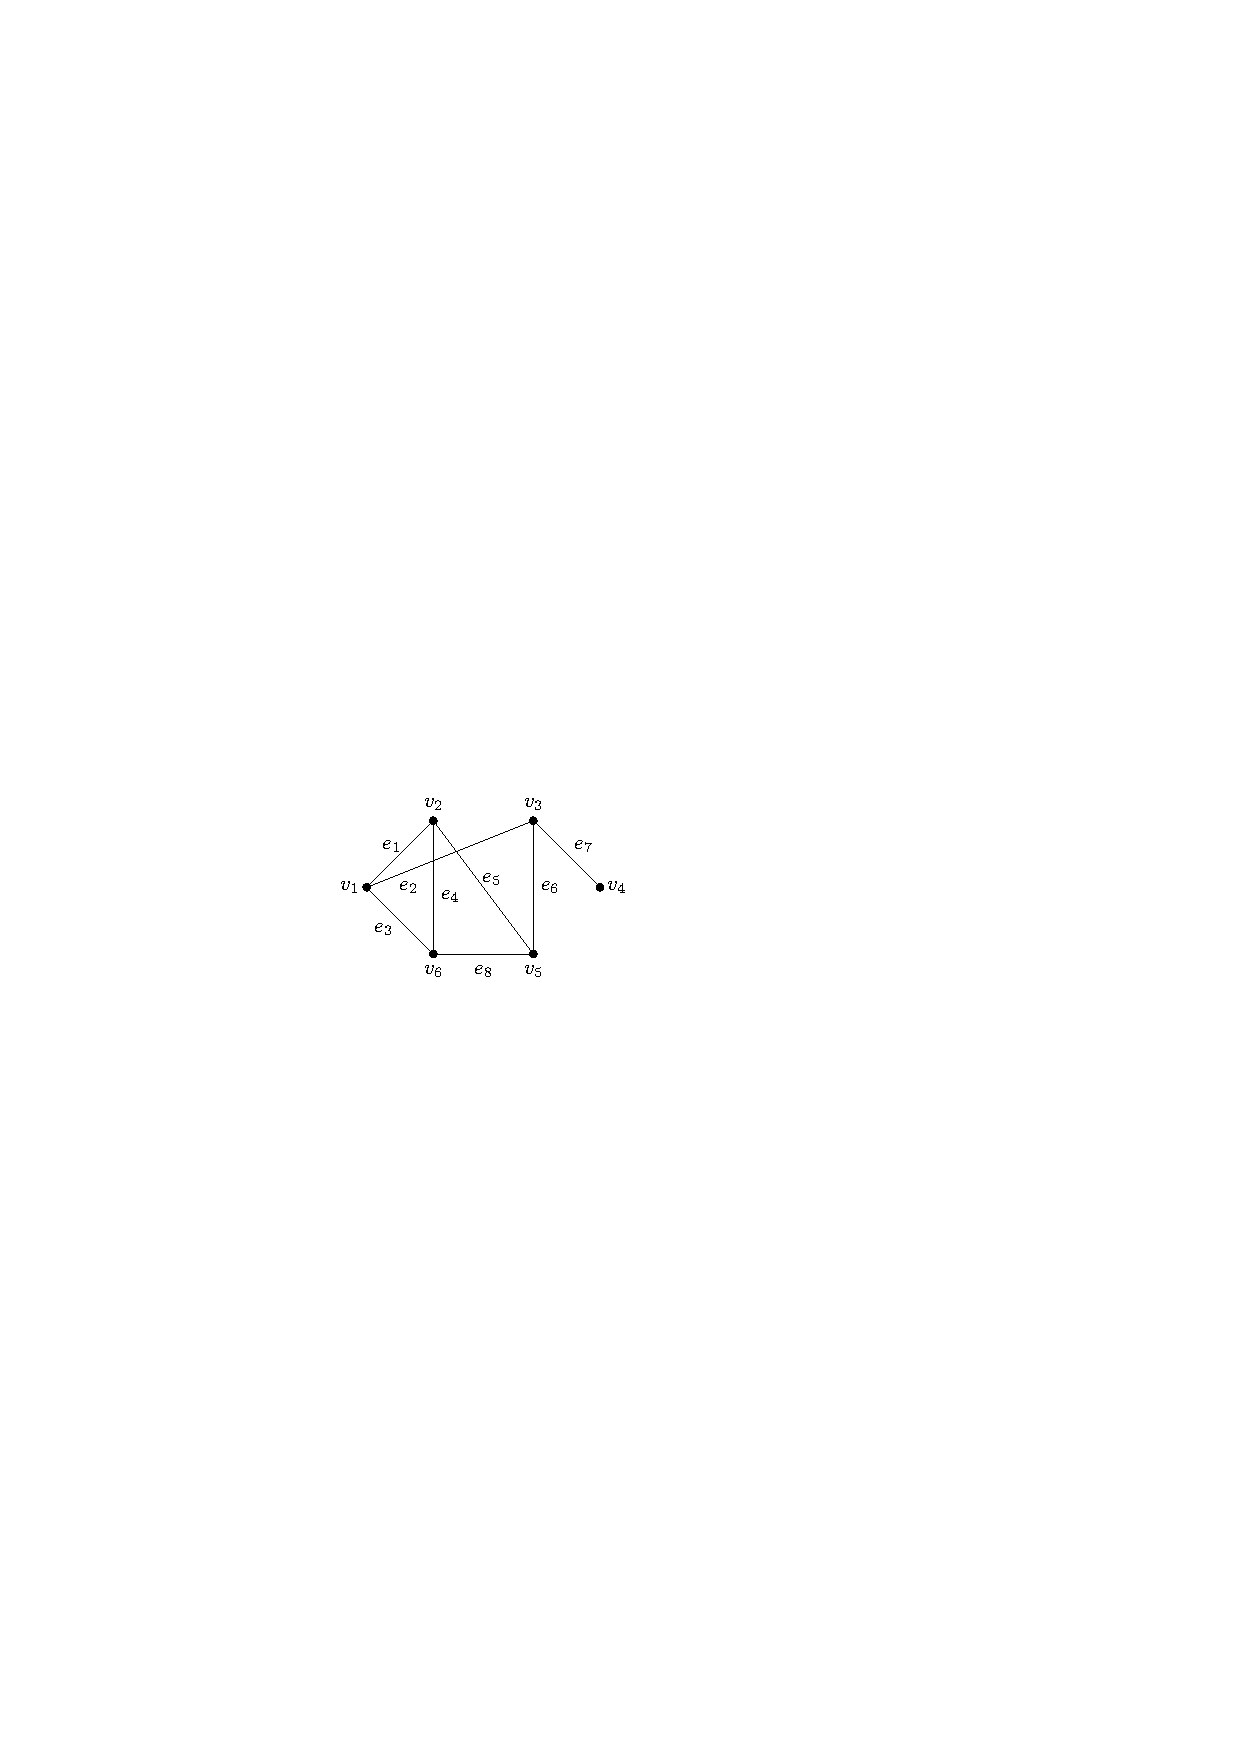
\includegraphics{Images/GNM(6,8).pdf}
\end{center}
is
\begin{equation*}
B = \begin{bmatrix}
1 & 1 & 1 & 0 & 0 & 0 & 0 & 0 \\
1 & 0 & 0 & 1 & 1 & 0 & 0 & 0 \\
0 & 1 & 0 & 0 & 0 & 1 & 1 & 0 \\
0 & 0 & 0 & 0 & 0 & 0 & 1 & 0 \\
0 & 0 & 0 & 0 & 1 & 1 & 0 & 1 \\
0 & 0 & 1 & 1 & 0 & 0 & 0 & 1 \\
\end{bmatrix}.
\end{equation*}
\end{Example}

Each column of the incidence matrix corresponds to an edge of the graph, and the only non-zero entries in the column correspond to the end-vertices of the edge -- thus, each column contains exactly two $1$s. In a simple graph, there is at most one edge between a given pair of vertices, and hence no two columns of the incidence matrix can be equal. We therefore have the following observation.

\begin{Observation}
The incidence matrix of a (simple, undirected) graph is a $0$-$1$ matrix in which every column has exactly two $1$s, and no two columns are equal.
\end{Observation}

\begin{Theorem}
If $B$ is the incidence matrix of a graph $G$, then the adjacency matrix of its line graph $L(G)$ is
\begin{equation*}
    A\pqty{L(G)} = B^T B - 2I
\end{equation*}
where $I$ is the identity matrix of order $|E(G)|$.
\end{Theorem}

\begin{proof}
Let $G$ be an $(n, m)$-graph with edge set $E = \{e_1, \ldots, e_m\}$. The incidence matrix $B = B(G)$ is of order $n \times m$, and therefore $B^T B - 2I$ (say) is of order $m \times m$.

Observe that the $(i, j)$ entry of $B^T B$ is the dot product of the $i$\nth and $j$\nth columns of $B$. As each column of $B$ has exactly two non-zero entries, both equal to $1$, the $(i, i)$ entry of $B^T B$ is $2$, and therefore the diagonal entries of $B^T B - 2I$ are all zero.

For $i \ne j$, the dot product of the $i$\nth and $j$\nth columns of $B$ will be $1$ if the edges $e_i$ and $e_j$ are adjacent (i.e., have one vertex in common), and $0$ otherwise -- note that the dot product cannot be $2$, as no two distinct columns of $B$ can be equal. Thus, for $i \ne j$, the $(i, j)$-entry of $B^T B$, which is equal to the $(i, j)$ entry of $B^T B - 2I$, is $1$ if and only if the edges $e_i$ and $e_j$ are adjacent in $G$, or equivalently, the vertices $e_i$ and $e_j$ of $L(G)$ are adjacent. Thus, $B^T B - 2I$ is the adjacency matrix of $G$.
\end{proof}

\section{Dijkstra's Algorithm}\label{sec:Dijkstra}

Let $G$ be a directed graph on $n$ vertices $v_1, \ldots, v_n$, in which each (directed) edge has a positive weight attached to it (say, representing the cost of traversing that edge). Let $W$ be the \newterm{weighted adjacency matrix} of $G$, defined as follows. $W$ is an $n \times n$ matrix with rows and columns indexed by the vertices of $G$, and having $(i,j)$-entry
\begin{equation*}
w_{ij} = \begin{cases}
0, & i = j\\
\text{Weight of the edge $(v_i, v_j)$}, & v_i \sim v_j\\
\infty, & v_i \not\sim v_j.
\end{cases}
\end{equation*}

Dijkstra's algorithm is a procedure to determine the shortest paths (and hence distances) from a given source vertex $s$ of $G$ to all the other vertices. 

\begin{algorithm}\caption{Dijkstra's algorithm}\label{alg:Dijkstra}
\begin{algorithmic}[1]
	\State $K \gets {s}$, $U \gets V(G) - \qty{s}$
	\State $\bestDTo(u) \gets w_{su}$, $\forall u \in U$
	\State $\tree(u) \gets s$, $\forall u \in U$
	\While{$|U| > 1$}
		\State $t \gets u \in U$ such that $\bestDTo(u)$ is minimum
		\State $U \gets U - \qty{t}$ \Comment{Remove $t$ from $U$ and}
		\State $K \gets K \cap \qty{t}$ \Comment{add it to $K$}
		\For{$u \in U$}
			\State $du_t \gets \bestDTo(t) + w_{tu}$ \Comment{Distance to $u$ through $t$}
			\If{$du_t < \bestDTo(u)$}
				\State $\bestDTo(u) \gets dsu_t$
				\State $\tree(u) \gets t$
			\EndIf
		\EndFor
	\EndWhile
\end{algorithmic}
\end{algorithm}


The input to the algorithm is the set of vertices $V$ and the weighted adjacency matrix $W$. Initially, the algorithm takes the weights of the edges from $s$ to the other vertices as the \newterm{tentative best distances} to those vertices. It also maintains a set $K$ of vertices to which the shortest paths from $s$ have been found (so that no further improvement is possible), and a set $U$ of vertices to which shorter paths may yet be found, passing through some vertex in $K$. In each step, the vertex $t \in U$ with minimum tentative best distance is selected -- it is guaranteed that no shorter path exists from $s$ to this vertex (since any such path would have to pass through some other vertex of $U$, but the distances to such a vertex is larger than the distance to $t$). This vertex $t$ is removed from $U$ and added to $K$, and then for each vertex $u$ remaining in $U$, the distance from $s$ to $u$ \emph{through} $t$ is compared with the current best distance to $u$. If the former is found to be smaller, the best distance to $u$ is updated to that value and $t$ is marked as the vertex through which $u$ is to be reached in the shortest path -- this is indicated by $\tree(u)$ in the algorithm. This procedure is repeated until there is only vertex remaining in $U$ (i.e., until $|U| = 1$).


\begin{Example}
In the graph shown below, find the shortest paths from $B$ to all the other vertices.\\
\begin{center}
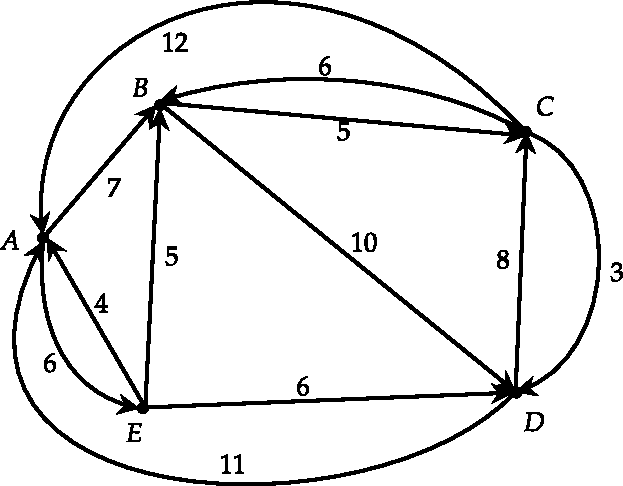
\includegraphics[scale=0.6]{Images/Dijkstra.pdf}
\end{center}
The weighted adjacency matrix of the graph is
\begin{equation*}
W = \kbordermatrix{
	&	A & B & C & D & E\\
	A & 0 & 7 & \infty & \infty & 6\\
	B & \infty & 0 & 5 & 10 & \infty\\
	C & 12 & 6 & 0 & 3 & \infty\\
	D & 11 & \infty & 8 & 0 & \infty\\
	E & 4 & 5 & \infty & 6 & 0
}.
\end{equation*}

The results of applying the algorithm are tabulated below and the tree of shortest paths is also shown.

\begin{center}
\begin{tabular}{cc}

	\begin{minipage}{5cm}
	$\begin{array}{r|cccc}
	 	 &		A	&	C	&	D	&	E\\
	\hline
	B(0) &	\infty_B	&	\boxed{5_B}	&	10_B	&	\infty_B\\
	C(5) &	17_C	&	\_	&	\boxed{8_C}	&	\infty_B\\
	D(8) &	\boxed{17_C}	&	\_	&	\_	&	\infty_B\\
	A(17)&	\_	&	\_	&	\_	&	23_A\\
	\hline
	B	&	17_C	&	5_B	&	8_C	&	23_A
	\end{array}$
	\end{minipage}
&
	\begin{minipage}{5cm}
		\centering
	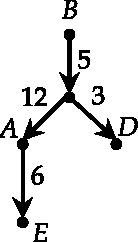
\includegraphics[scale=0.7]{Images/ShortestPaths.pdf}
	\end{minipage}

\end{tabular}
\end{center}

\end{Example}

\section{Prim's Algorithm}\label{sec:Prim}

Let $G$ be a weighted, undirected, connected graph with positive edge weights. A \newterm{minimal spanning tree} of $G$ is a spanning tree $T$ of $G$ such that the sum of the weights of its edges is minimum among all the spanning trees of $G$.

\begin{algorithm}\caption{Prim's algorithm}\label{alg:Prim}
\begin{algorithmic}[1]
\Require{Weighted, undirected, connected graph $G$, source vertex $v \in V(G)$}
	\State $V(T) \gets \{v\}$, $E(T) \gets \varnothing$
	\While{$V(T) \ne V(G)$}
        \State $e \gets$ minimum-weight edge with one end-vertex in $V(T)$ and one end-vertex not in $V(T)$
        \State $E(T) \gets E(T) \cup \{e\}$
        \State $V(T) \gets V(T) \cup \{x, y\}$ where $e = xy$
	\EndWhile
\end{algorithmic}
\end{algorithm}

\begin{Example}
Apply Prim's algorithm to the graph given below to obtain a minimal spanning tree. Take $v_1$ as the initial vertex.
\begin{center}
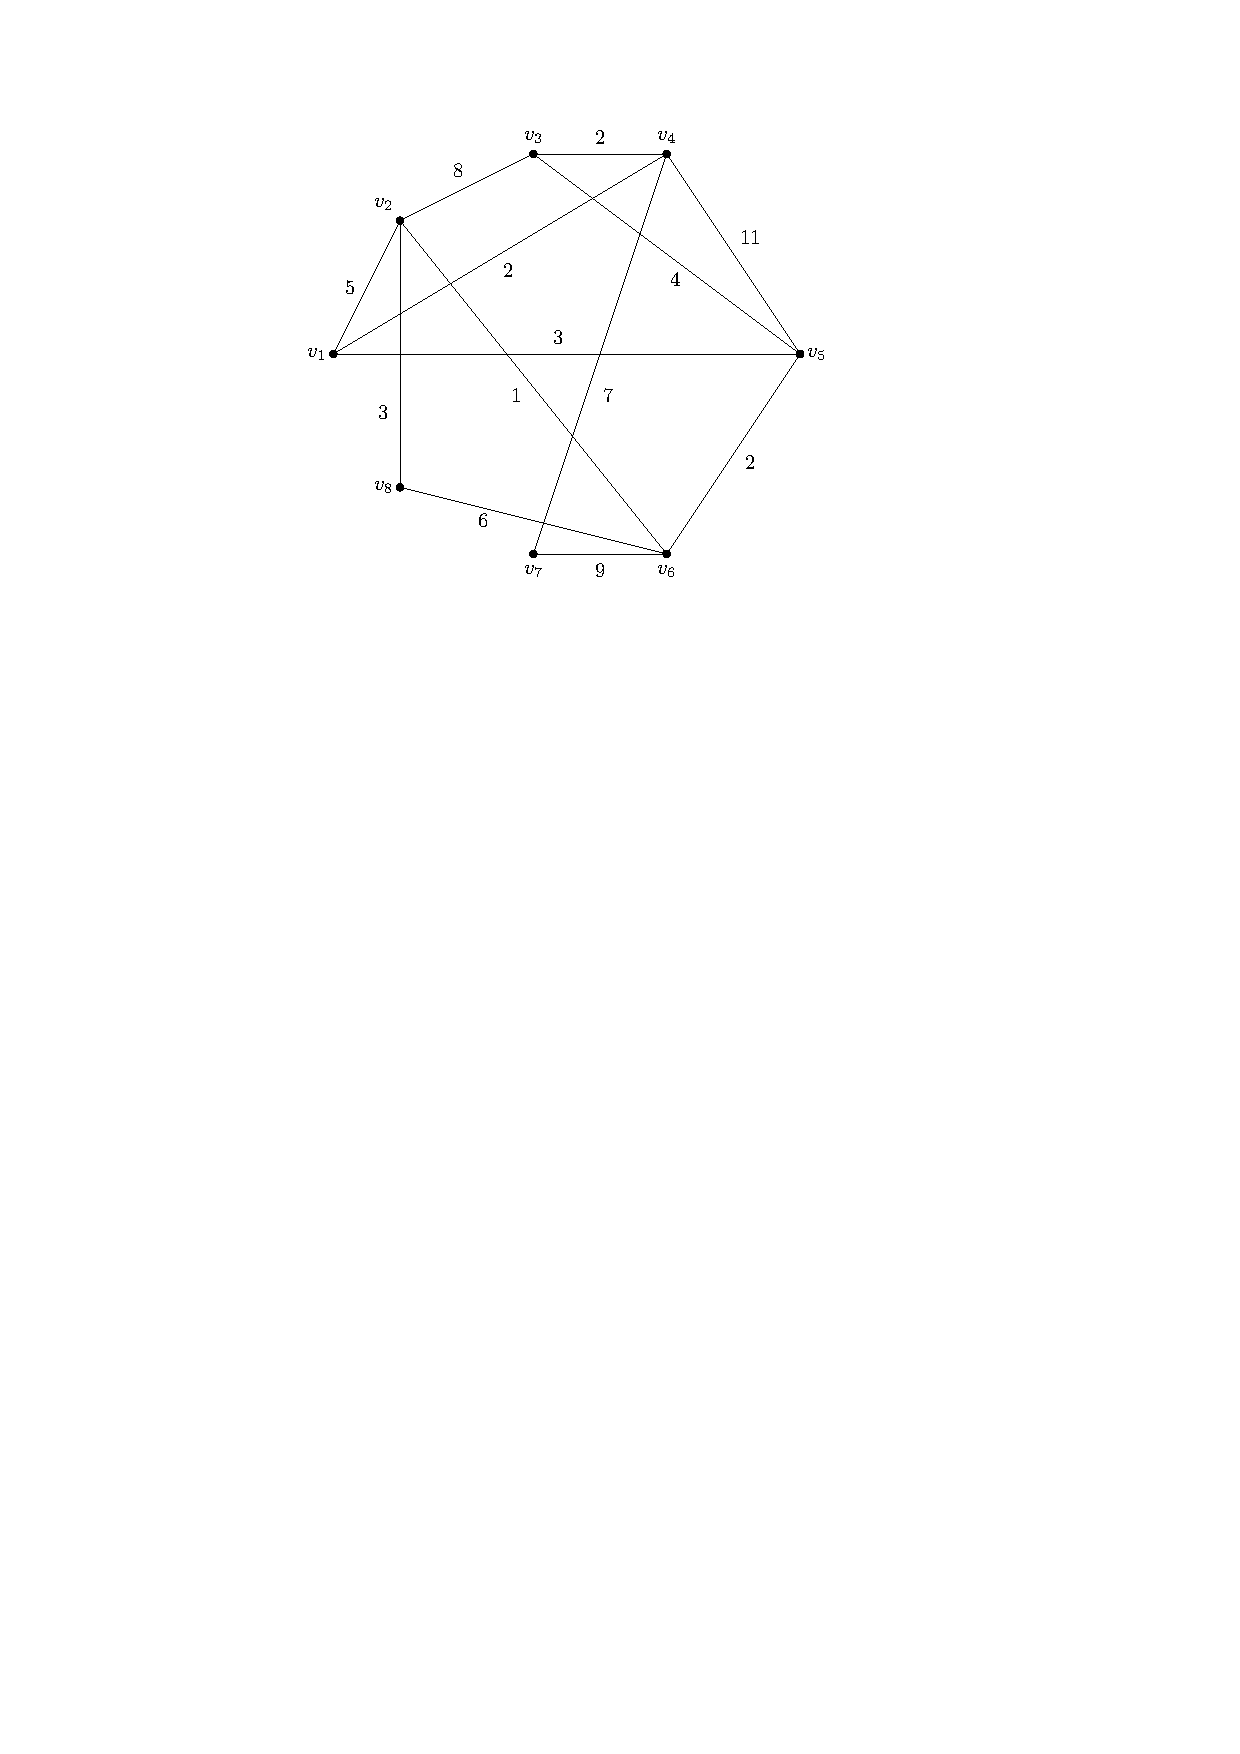
\includegraphics{Images/Prim.pdf}
\end{center}
\vspace{1em}
The step-by-step result of the algorithm is tabulated below.
\begin{center}
\def\arraystretch{1.3}
\begin{tabular}{c|>{\centering\arraybackslash}p{0.4\textwidth}|>{\centering\arraybackslash}p{0.2\textwidth}|c}
Step & Edge added & Vertex added & Total weight \\
\hline
1 & $-$ & $v_1$ & $0$ \\
2 & $(v_1, v_4)$ & $v_4$ & $2$ \\
3 & $(v_4, v_3)$ & $v_3$ & $4$ \\
4 & $(v_1, v_5)$ & $v_5$ & $7$ \\
5 & $(v_5, v_6)$ & $v_6$ & $9$ \\
6 & $(v_6, v_2)$ & $v_2$ & $10$ \\
7 & $(v_2, v_8)$ & $v_8$ & $13$ \\
8 & $(v_4, v_7)$ & $v_7$ & $20$ \\
\end{tabular}
\end{center}
\vspace{1em}
Therefore, the minimal spanning tree is:
\begin{center}
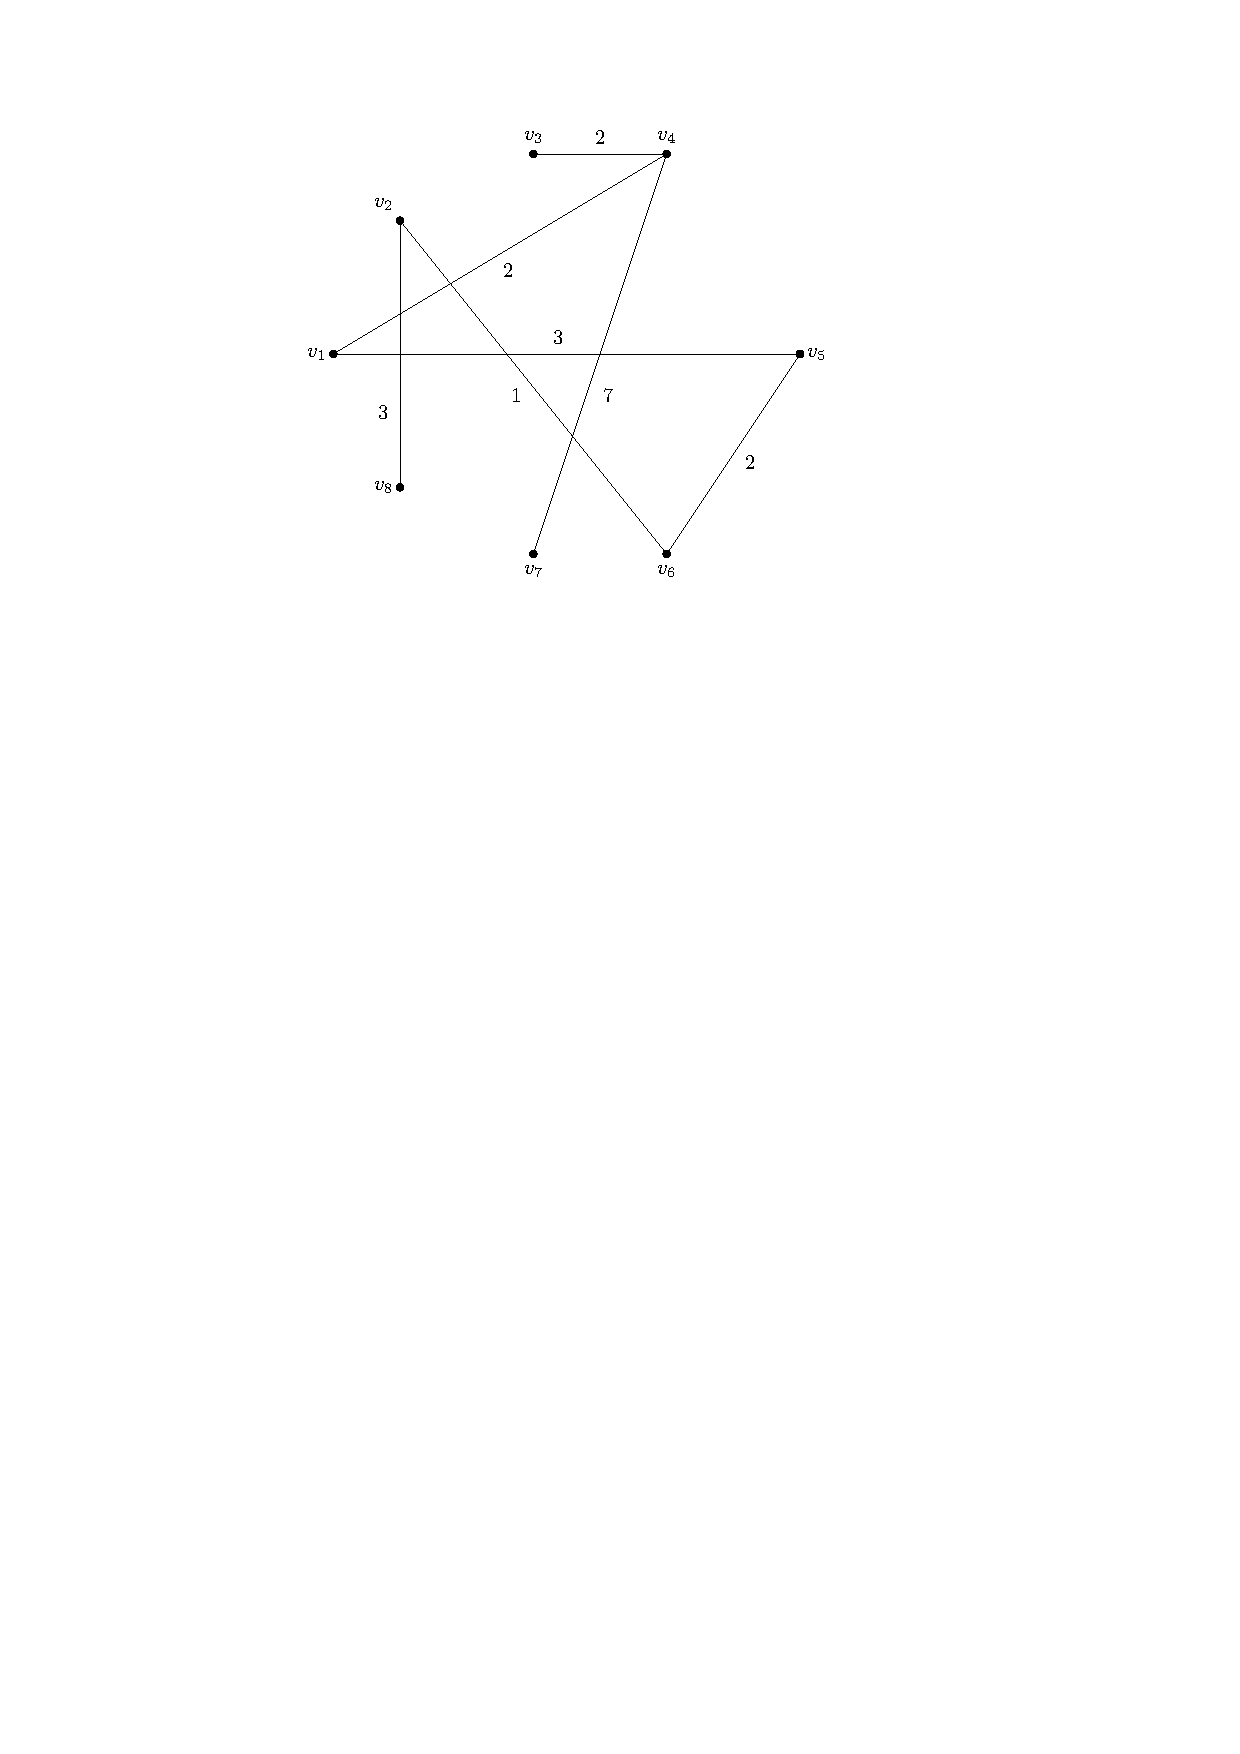
\includegraphics[scale=0.8]{Images/MST.pdf}
\end{center}
\end{Example}

%\begin{appendices}
%
%\end{appendices}